\chapter{Ray tracing}\label{chap:raytracing}
Optical ray tracing is a tool to calculate the transport of light within optical systems.
Given an optical system and a set of rays at the source, ray tracing relates the emitted light with its output distribution. 
The influence of diffraction on the transport of a ray is neglected. \\ \indent
Although the method can be implemented for two or more dimensions and for any optical system, here we consider the two-dimensional case only. 
We will thus refer to optical lines instead of optical surfaces.
The two-dimensional case has some limitations. For example, it may not identify skew rays that are turned back by the system, with the consequence that a 2D analysis cannot guarantee a proper treatment of non-meridional rays in 3D. 
Nevertheless, the two-dimensional case is particularly relevant because it is a good test case to demonstrate the performance of new methods.
Optical designers often start with 2D systems, where only the meridional plane is taken into account because it gives a good prediction of the target distribution of the rays
(see \cite{winston2005nonimaging}, chapter $4$).
% Why there are alternatives
\section{Ray tracing for two-dimensional optical systems}\label{sec:raytracing}
The purpose of ray tracing applied to non-imaging optical systems is to calculate the target rays distribution given an optical system and an initial distribution of the rays at the source.
Light rays are straight lines and they are reflected or refracted by the optical components of a system.
Every ray emitted from the source is followed until it reaches the target.  
The ray tracing procedure is constructed such that the position and the direction of the rays are calculated on every optical line that they hit. \\ \indent
Given a Cartesian coordinate system $(\variabile{x}, \variabile{z})$, a two-dimensional optical system symmetric with respect to the $\variabile{z}$-axis is defined.
Hence, we assume that the optical axis coincides with the $\variabile{z}$-axis.
The optical system is formed by a source \point{S}, a target  \point{T} and some optical components labeled with indexes $\lineai$ where $\lineai \in \{2, \cdots, \nline-1\}$ and $\nline$
 indicates the number of lines that form the system. \point{S} and \point{T} are indicated with the indexes $1$ and $\nline$, respectively.
The index of refraction of the medium in which line $\lineai$ is located is indicated with $\n_\lineai$.
Every ray emitted by \point{S} (line $1$) can hit some optical components $\lineai\in\{2, \cdots, \nline -1\}$ before reaching \point{T} (line $\nline$).
The intersection point of the rays with line $\lineai$ are $(\variabile{x}_\lineai, \variabile{z}_\lineai)_{\lineai =1, \cdots, \nline}$ and, $\vect{s}_\lineai= (-\sin \optangle_\lineai, \cos \optangle_\lineai)$ indicates the direction vector of the rays that leave $\lineai$,
with $\optangle_\lineai$ the angle that the ray forms with respect to the optical axis measured counterclockwise. As we consider only forward rays, the angles
$\optangle_\lineai\in (-\pi/2, \pi/2)$.
Therefore, a ray segment between $(\variabile{x}_\lineai, \variabile{z}_\lineai)$ and $(\variabile{x}_\lineaj, \variabile{z}_\lineaj)$
with $\lineaj\neq\lineai$ is parameterized in real space by:
\begin{equation}
\label{parametrization}
\vect{r}(\variabile{s})=
\left( \begin{array}{cc}
\variabile{x}_\lineai-\variabile{s}\sin\optangle_\lineai \\
\variabile{z}_\lineai+\variabile{s}\cos\optangle_\lineai\end{array} \right) \qquad \quad 0< \variabile{s}\leq \variabile{s}_{\textrm{max}}\,,
\end{equation}
where \variabile{s} denotes the arc-length and $\variabile{s}_{\textrm{max}}$ is the maximum value that it can assume.
Figure \ref{fig:cup} shows an example where a single ray is traced inside a very simple optical system, the so-called two-faceted cup.
\begin{figure}[t]
\label{fig:cup}
  \begin{center}
%\vspace{-1.5cm}
  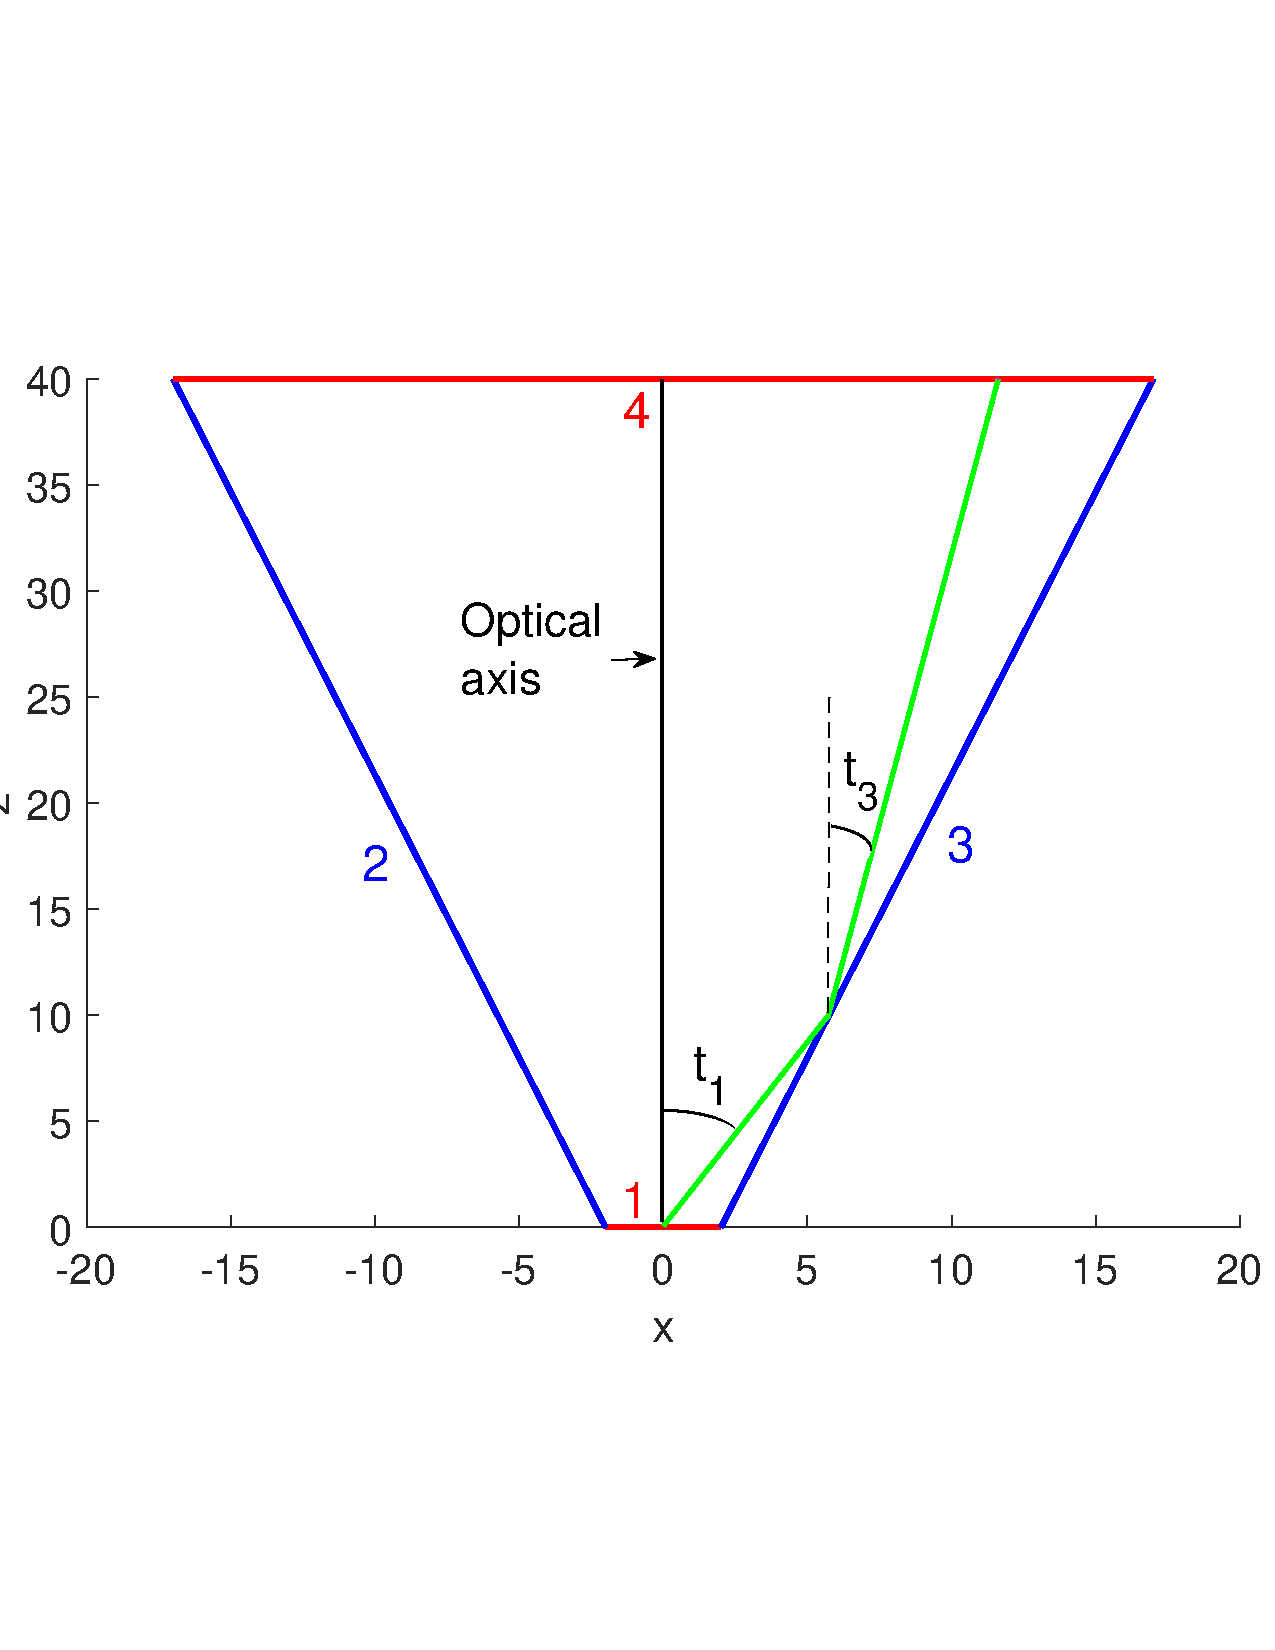
\includegraphics[width=6.7cm]{cup.pdf}
  \end{center}
%\vspace{-2cm}
  \caption{\textbf{Shape of the two-faceted cup.}  Each line of the system is labeled with a number.
   The source \point{S}$= [-2,2]$ (line number $1$) is located on the $\variabile{x}$-axis.
   The target \point{T}$= [-17, 17]$ (line $4$) is parallel to the source and is located at a height $\variabile{z}= 40$.
   The left and right reflectors (line $2$ and $3$) connect the source with the target.}
  \label{fig:cup}
\end{figure}
The light source \point{S}$= [-\variabile{a}, \variabile{a}]$ (line $1$) and the target \point{T}$~=~ [-\variabile{b}, \variabile{b}]$ (line $4$) are two segments normal to the \variabile{z}-axis, where $\variabile{a}=2$ and $\variabile{b}=17$.
The left and right reflectors (line $2$ and $3$) are oblique segments that connect the source and the target.
All the optical lines $\lineai \in \{1, \cdots, 4\}$  are located in air, thus the refractive index is $\n_{\lineai}=1$ for every $\lineai$. \\ \indent
In order to compute the target photometric variables, we need to know how the optical system influences the direction of the rays when they hit an optical line.
Ray tracing relates the position coordinates
 $ (\variabile{x}_1, \variabile{z}_1)$ and the direction vector $\vect{s}_1$ of every ray at the source $\point{S}$ with the corresponding position $(\variabile{x}_\nline, \variabile{z}_\nline)$ and direction $\vect{s}_\nline$
 at the target $\point{T}$. In the following we will often use the target coordinates of the rays thus, to simplify the notation, we do not write the subscript $\nline$ for the target coordinates. We rather write $(\variabile{x},\variabile{z})$ instead of $(\variabile{x}_\nline, \variabile{z}_\nline)$,  $\optangle$ instead of $\optangle_\nline$ and $\vect{s}$ instead of $\vect{s}_{\nline}$ for the target coordinates.
The ray tracing algorithm can be outlined as follows:
\begin{enumerate}
\item Indicating with $\variabile{i}$ the index of the line that rays leave, start considering a ray thet leaves the source $\point{S}$ (line \variabile{i}=1);
 \item Consider a ray with position coordinates $(\variabile{x}_\variabile{i}, \variabile{z}_\variabile{i})$ and direction $\vect{s}_\variabile{i}~=~(-\sin \optangle_\variabile{i}, \cos \optangle_\variabile{i})$, use Equation ($\ref{parametrization}$) to implement the ray parametrization $\vect{r}(\variabile{s}_\variabile{i})$;
\item Compute the coordinates $(\variabile{x}_\variabile{k}, \variabile{z}_\variabile{k})_{\variabile{k} = 1\cdots, \nline}$ of the intersection point of the parameterized ray $\vect{r}(\variabile{s})$ with all the lines that it crosses
\begin{itemize}
\item[a)] if the shape of the lines is described by an explicit equation, the intersection points are determined analytically;
\item[b)] if there is no analytic description for the optical lines, the intersections need to be determined using iterative methods;
\end{itemize}
\item  Determine the minimal positive distance between $(\variabile{x}_\variabile{i}, \variabile{z}_\variabile{i})$ and $(\variabile{x}_\variabile{k}, \variabile{z}_\variabile{k})$ for every $\variabile{k}=1, \cdots, \nline$.
\item Indicate with $\lineaj$ the line for which its intersection with the ray is located at the minimal distance form $(\variabile{x}_\variabile{i}, \variabile{z}_\variabile{i})$;
\item If $\lineai = \nline$, stop the procedure, the target ray's coordinates $(\variabile{x}, \variabile{z})$ and $\vect{s}$ are found.
\item If $\lineai \neq \nline$, calculate the normal $\boldsymbol{\nu}_\lineai$ to line $\lineai$ at the point $(\variabile{x}_{\lineai}, \variabile{z}_{\lineai})$;
 \item Compute the new ray direction $\vect{s}_\lineai$ of the ray that leaves line $\lineai$ at the point $(\variabile{x}_{\lineai}, \variabile{z}_{\lineai})$:
\begin{itemize}
\item[a)] if the incident line is a reflective line, $\vect{s}_\lineai$ is given by Eq. (\ref{Reflection});
\item[b)] if the incident line is a refractive line, $\vect{s}_\lineai$ is given by Eq. (\ref{Refraction});
\end{itemize}
\item Put $\variabile{i}=\lineai$ and restart the procedure from $2.$
\end{enumerate}
% The goal intensity
% Same approach of computing an integral
% How to chose the initial rays at the source
The procedure explained above is repeated for every ray traced through the system, \cite{Gross2005Handbook}. 
Once the target position and the direction of every ray traced are computed, the target photometric variables can be calculated using the definitions explained in the previous chapter, see Section \ref{sec:photometry}.
% Put the algorithm
\\ \indent
There are different ways to implement the ray tracing procedure. The efficiency of the ray tracing can be related to the distribution of the rays at the source. 
If the initial position and direction of the rays are chosen randomly we have Monte Carlo (MC) ray tracing. 
This is a very common method in non-imaging optics as it is very powerful and easy to implement. MC ray tracing will be explained in detail in the next paragraph.
If the rays are chosen from a so-called low discrepancy sequence we have Quasi-Monte Carlo (QMC) ray tracing.
This approach is discussed in Section \ref{sec:QMC}.
\section{Monte Carlo ray tracing}
As explained above, the aim of ray tracing is to calculate the target photometric variables given an initial light distribution at the source. To this purpose, we can think of a light source as
emitting a very large number of random rays and keep track of where they go. In this way we can calculate, for instance the target luminance distribution. Next the target intensity is given by the integral of the luminance (see Equation \ref{eq:int_lum}) which can be approximated by the average of the luminance values. This simple method uses the same idea of a family of techniques called Monte Carlo simulation and can be a very easy way to numerically
solve physics problems based on numerical integration \cite{jensen2003monte}.
\\ \indent Before explaining the details of MC ray tracing, we give an introduction to MC methods for the two-dimensional case. Let us consider a set $D = [\vect{a}, \vect{b}]$ with $\vect{a} = (a_1, a_2)$ and $\vect{b} = (b_1, b_2)$ elements of $\mathbb{R}^2$ such that
$[\vect{a}, \vect{b}]  = [a_1, b_1] \times [a_2, b_2]$. Consider function $f:[\vect{a},\vect{b}]\subset \mathbb{R}^2 \mapsto \mathbb{R}$ and a random variable 
$\vect{Y}$ with values in $D$ with probability density function $\rho(\vect{y})$, where $\vect{y}$ are the values $\vect{Y}$ in $D$. Note that we indicate the random variables with capital letters and the corresponding deterministic values with lowercase letters. The expected value of $f$ with respect of $\rho$ is:
\begin{equation}
\mathbb{E}[f] =\int_{D}f(\vect{y})\rho(\vect{y}) \textrm{d}\vect{y}.
\end{equation}
If $\rho$ is a uniform probability density function, the expected value is given by:
\begin{equation}\label{eq:expected_value}
\mathbb{E}[f] =\frac{1}{\lambda([\vect{a},\vect{b}])} \int_{D}f(\vect{y}) \textrm{d}\vect{y},
\end{equation}
where $\lambda([\vect{a},\vect{b}]) = (b_1-a_1)\times (b_2-a_2)$.
Monte Carlo method approximates the integral in Equation (\ref{eq:expected_value}) by the sum:
\begin{equation}
S_{N}[f] = \frac{1}{N} \sum_{\variabile{i}=1}^{N} f(\vect{Y}_\variabile{i}),
\end{equation}
where $\{\vect{Y}_\variabile{i}\}_{\variabile{i} = 1, \cdots, \const{N}}$ are independent samples of the probability density function $\rho$ with values in $D$ \cite{owen2003quasi}. Thus, MC is based on the following approximation:
\begin{equation}\label{eq:approx_MC_QMC}
\int_{D}f(\vect{y})\rho(\vect{y}) \textrm{d}\vect{y}\approx\frac{1}{N} \sum_{\variabile{i}=1}^{N} f(\vect{Y}_\variabile{i}).
\end{equation}
According to the strong law of large numbers,
\begin{equation}
\const{Pr}\Big(\lim_{N\rightarrow\infty}\frac{1}{N}\sum_{\variabile{i}=1}^{N} f(\vect{Y}_\variabile{i}) = \mathbb{E}[f(\vect{Y})] \Big) = 1.
\end{equation}
Therefore, for sufficiently large $N$ the expected value of $f$ is approximated by the empirical mean:
\begin{equation}
\mathbb{E}[f] \approx \frac{1}{N} \sum_{\variabile{i}=1}^{N} f(\vect{Y}_\variabile{i}).
\end{equation}
From the linearity of the expected value\footnote{Given a set of independent random variables $\{X_\variabile{i}\}_{\variabile{i}=1, \cdots, N}$ and a real number $a$, the expected value satisfies:
$\mathbb{E}\big[\sum_{\variabile{i}=1}^{N}X_{\variabile{i}}\big] = \sum_{\variabile{i}=1}^{N}\mathbb{E}[X_{\variabile{i}}]$ and $\mathbb{E}[a\,X_\variabile{i}] = a\mathbb{E}[X_{\variabile{i}}]$.},
 it follows
\begin{equation}\label{eq:linearity}
\mathbb{E}[S_{N}(f)] = \frac{1}{N}\sum_{\variabile{i}=1}^{\textrm{N}}\mathbb{E}[f(\vect{Y}_{\variabile{i}})] = \mathbb{E}[f(\vect{Y})],
\end{equation}
while the Bienaym\'e formula\footnote{Given a set of \textit{independent} random variables $\{X_\variabile{i}\}_{\variabile{i}=1, \cdots, N}$ and a real number $a$, the variance satisfies:
$\textrm{Var}\big[\sum_{\variabile{i}=1}^{N}X_{\variabile{i}}\big] = \sum_{\variabile{i}=1}^{N}\textrm[X_{\variabile{i}}]$ and $\textrm{Var}[a\,X_\variabile{i}] = a^2\textrm{Var}[X_{\variabile{i}}]$.} leads to
\begin{equation}\label{eq:variance}
\textrm{Var}[S_{N}]= \textrm{Var}\Bigg[\frac{1}{N}\sum_{\variabile{i}=1}^{N}f(\vect{Y}_\variabile{i})\Bigg] =
 \frac{1}{N^2}\sum_{\variabile{i}=1}^{N}\textrm{Var}\big[f(\vect{Y}_\variabile{i})\big] = \frac{1}{N}Var[f(\vect{Y})]
\end{equation}
which can be applied because the random variables $\{\vect{Y}_\variabile{i}\}_{i = 1, \cdots, N}$ are independent \cite{grinstead2012introduction}. 
Suppose that $f$ has variance $\textrm{Var}[f]=\mathbb{E}[(f-\mathbb{E}(f))]^2 = \sigma^2[f] $, Equations (\ref{eq:linearity}) and (\ref{eq:variance}) give
\begin{equation}\label{eq:variance2}
\textrm{Var}[S_N(f)] = \mathbb{E}[(S_{N}(f)-\mathbb{E}[S_{N}(f)])^2]= \mathbb{E}[(S_{N}(f)-\mathbb{E}[f])^2] = \sigma^2[f]/N.
\end{equation}
Let us denote the integration error with:
\begin{equation}\label{eq:error1}
\const{err}(f, S_{\const{N}}) =\int_{D}f(\vect{y})\rho(\vect{y}) \textrm{d}\vect{y}-S_{\const{N}}(f) = \mathbb{E}[f]-S_\const{N}(f).
\end{equation}
Considering a convex function $g:\variabile{x}\in D\mapsto\variabile{x}^2$ we can write:
\begin{equation}
\begin{aligned}
&\mathbb{E}[|\const{err}(f, S_{\const{N}})|] = \sqrt{\mathbb{E}[|\const{err}(f, S_{\const{N}})|^2]} = \sqrt{g\big(\mathbb{E}[|\const{err}(f, S_{\const{N}})|]\big)}) \\&\leq\sqrt{\mathbb{E}[g(|\const{err}(f, S_{\const{N}})|]}) = \sqrt{\mathbb{E}[\const{err}^2(f, S_{\const{N}})]})
\end{aligned}
%\begin{aligned}
%\mathbb{E}\big[|\const{err}(f, S_{\const{N}})|\big] &= \frac{1}{\const{N}}\sqrt{\Bigg(\sum_{\variabile{1}=1}^\const{N}|\const{err}(f, S_{\const{N}})|\Bigg)^2}  \leq \frac{1}{\const{N}}\sqrt{\const{N}\sum_{\variabile{1}=1}^\const{N}\big(\const{err}(f, S_{\const{N}})\big)^2}  \\
%& =\sqrt{\frac{1}{\const{N}}\sum_{\variabile{1}=1}^\const{N}\big(\const{err}(f, S_{\const{N}})\big)^2}= \sqrt{\mathbb{E}\big[\const{err}(f, S_{\const{N}})^2\big]}
%\end{aligned}
\end{equation} 
where the inequality follows from the Jensen's inequality (\cite{williams1991probability} Chapter $6$).
Using the previous relation and Equations (\ref{eq:variance2}) and (\ref{eq:error1}), we obtain:
\begin{equation}\label{eq:mean_error}
\mathbb{E}\big[|\const{err}(f, S_{\const{N}})|\big]\leq
\sqrt{\mathbb{E}\big[\const{err}(f, S_{\const{N}})^2\big]} = \frac{\sigma[f]}{\sqrt{\const{N}}},
\end{equation}
Hence, the absolute value of the integration error is, on average, bounded by $\sigma[f]/\sqrt{\const{N}}$, where $\sigma[f]$ is the standard deviation of $f$ \cite{leobacher2014introduction}. It is very important to note that $\const{err}(f, S_{\const{N}})$ does not depend on the dimension of $f$.
\\ \indent The MC technique can be combined with ray tracing procedure in order to compute the light distribution at the target of an optical system.
In MC ray tracing the position and the direction of  every ray at the source are chosen randomly. 
In the two-dimensional case, for every ray we need to choose one position coordinate $\variabile{x}_1$ and one angular coordinate $\optangle_1$ at the source, while the $\variabile{z}_1$ coordinate of every ray at the source is always given (for instance, for the two-faceted cup in Figure \ref{fig:cup}, $\variabile{z}_1=0$ for every ray). 
Indicating with $\variabile{x}_{1}^{\variabile{i}}$ $\variabile{x}$-coordinate of the $\variabile{i}$-th ray and with $\optangle_1^{\variabile{i}}$ its angular coordinate, a set of random variables $\{\vect{Y}_1, \cdots, \vect{Y}_N\}\in [\vect{a}, \vect{b}]\subset\mathbb{R}^2$ is chosen such that $\vect{Y}_{\variabile{i}}= (\variabile{x}_{1}^{\variabile{i}},\optangle_1^{\variabile{i}})$.
% the initial position coordinate $\variabile{x}_1$ of the $\variabile{k}$-th ray corresponds to the first component of the $\variabile{k}$-th random variable $\vect{y}_\variabile{k}$ and, the starting angular coordinate $\optangle_1$ of the $\variabile{k}$-th ray corresponds to the second component of the $\variabile{k}$-th random variable $\vect{y}_\variabile{k}$.
Rays with those random coordinates at \point{S} are traced from \point{S} to \point{T} and, a probabilistic interpretation of the output photometric variables is provided.
In particular, we are interested in the target intensity $I$ as a function of the angular coordinate $\optangle$. Using the idea of MC method we approximate its expected value $\mathbb{E}[I]$ by a sum as described in Equation (\ref{eq:approx_MC_QMC}) where the function $f$ is now the intensity $I$.
%which is given by:
%\begin{equation}\label{eq:MC_intensity}
%I(\optangle) = \int_{\variabile{x}^{\textrm{min}}}^{\variabile{x}^{\textrm{max}}}L(\variabile{x}, \optangle)\textrm{d}\variabile{x}\,
%\end{equation}
%where $\variabile{x}^{\textrm{min}}$ and $\variabile{x}^{\textrm{max}}$ are the minimum and the maximum position coordinates of the rays at the target. Using the MC average, the previous integral is approximated by:
%\begin{equation}\label{eq:MC_approximated_lum}
%\int_{\variabile{x}^{\textrm{min}}}^{\variabile{x}^{\textrm{max}}}L(\variabile{x}, \optangle)\textrm{d}\variabile{x} \approx \frac{1}{N}\sum_{\variabile{i}=1}^{N}L(\variabile{x}^{\variabile{i}}, \optangle^{\variabile{i}}).
%\end{equation}
\\ \indent The idea is to divide the target into intervals of equal length, the so-called bins and counting on average the number  of rays that fall into each bin. 
In the following we explain how the value of the intensity in each bin is calculate and we provide an estimation of the MC error over every bin. \\ \indent A partitioning
$P_1: -\pi/2 = \optangle_{0}<\optangle_{1}<\cdots <\optangle_{\nbin}=\pi/2$ of the interval $[-\pi/2, \pi/2]$ is defined where $\nbin$ is the number of bins in $P_1$.
We remark that, with a slight abuse of notation, we indicated the angular coordinates of the rays at the target (line $\nline$) with $\optangle_{\variabile{j}}$ instead of $\optangle_{\nline,\variabile{j}}$ for every $\variabile{j}\in\{0, \cdots, \nbin\}$. 
The normalized approximated intensity $\hat{I}_{\const{MC}}(\optangle)$ is a piecewise constant function, whose value over the $\variabile{j}$-th bin is the ratio between the number of rays that fall into that bin
$\const{Nr}[\optangle_{\variabile{j}-1},\optangle_{\variabile{j}})$ and the total number of rays traced $\const{Nr}[-\pi/2, \pi/2)$.
The averaged normalized MC intensity $\hat{I}_{\const{MC}}$ in a single bin is defined by:
\begin{equation} \label{g_mc}
\hat{I}_{\const{MC}}(\optangle) = \frac{\const{Nr}[\optangle_{\variabile{j}-1},\optangle_{\variabile{j}})}{\const{Nr}[-\pi/2, \pi/2)} \qquad \mbox{ for } \optangle\in[\optangle_{\variabile{j}-1}, \optangle_{\variabile{j}}).
\end{equation}
The output intensity is computed from the value of the intensity $I_{\const{MC}}(\optangle_{\variabile{j}-1/2})$ along the direction $\optangle_{\variabile{j}-1/2}=(\optangle_{\variabile{j}-1}+
\optangle_{\variabile{j}})/2$ for every bin $[\optangle_{\variabile{j}-1},\optangle_{\variabile{j}})_{\variabile{j} = 1, \cdots, \nbin}$.
 The intensity $I_{\const{MC}}(\optangle_{\variabile{j}-1/2})$ gives an estimate of the probability that a ray reaches the target with an angle in the $\variabile{j}$-th interval
$[\optangle_{\variabile{j}-1}, \optangle_{\variabile{j}})$ of the partitioning $P_1$. This probability $\const{P}_{\variabile{j}, \Delta\optangle}$ is given by
\begin{equation}\label{eq:probability}
\const{P}_{\variabile{j}, \Delta\optangle} = \Pr(\optangle_{\variabile{j}-1}\leq\optangle<\optangle_{\variabile{j}})=
\frac{\int_{\optangle_{\variabile{j}-1}}^{\optangle_{\variabile{j}}} I(\optangle) \textrm{d}\optangle}{\int_{-\pi/2}^{\pi/2}I(\optangle) \textrm{d}\optangle}\,,
\end{equation}
where $I(\optangle)$ is the output intensity (not normalized).
Note that $\sum_{\variabile{j}=1}^{\nbin}\const{P}_{\variabile{j}, \Delta\optangle}=1$. From the mean value theorem for the function
$I(\optangle)$, which is continuous in $[\optangle_{\variabile{j}-1}, \optangle_{\variabile{j}}]$, there exists a value $\optangle_{\variabile{j}}\in[\optangle_{\variabile{j}-1}, \optangle_{\variabile{j}}]$ for which:
 \begin{equation}\label{eq:deltatI}
\int_{\optangle_{\variabile{j}-1}}^{\optangle_{\variabile{j}}} I(\optangle) \textrm{d}\optangle = \Delta \optangle\;I(\optangle_{\variabile{j}}).
\end{equation}
Hence, $\const{P}_{\variabile{j}, \Delta\optangle}$ is proportional to the size $\Delta\optangle= (\optangle_{\nbin}-\optangle_{0})/{\nbin}$
of the bins and to $I(\optangle_{\variabile{j}})$. Although $I(\optangle_{\variabile{j}})$ does depend on the number of bins \nbin, it is taken constant as it is the value of the intensity on a given direction\footnote{This is possible since $I(\optangle_{\variabile{k}})$ is a continuous function in the closed interval $[\optangle_{\variabile{j}-1}, \optangle_{\variabile{j}}]$.}, so Equation (\ref{eq:deltatI}) proves that $\const{P}_{\variabile{j}, \Delta\optangle}$ is inversely proportional to the number of bins $\nbin$ of the partitioning $P_1$.
Indicating with $\Phi = \int_{-\pi/2}^{\pi/2}I(\optangle) \textrm{d}\optangle$ the total flux (measured in lumen, $\textrm{lm}$),
the error between the intensity $I(\optangle_{\variabile{j}-1/2})$
 and the averaged \const{MC} intensity $\Phi I_{\const{MC}}(\optangle_{\variabile{j}-1/2})/\Delta\optangle$ is given by
\begin{equation}\label{eq:error_int}
\begin{aligned}
\Big|I(\optangle_{\variabile{j}-1/2})&-\frac{\Phi}
{\Delta\optangle}I_{\const{MC}}(\optangle_{\variabile{j}-1/2})\Big| \leq\\
 &\Big|I(\optangle_{\variabile{j}-1/2})-\frac{1}{\Delta \optangle}\int_{\optangle_{\variabile{j}-1}}^{\optangle_{\variabile{j}}} I(\optangle)\textrm{d}\optangle\Big|+\\
&\frac{1}{\Delta \optangle}\Big|\int_{\optangle_{\variabile{j}-1}}^{\optangle_{\variabile{j}}} I(\optangle)\textrm{d}\optangle-
\Phi\, I_{\const{MC}}(\optangle_{\variabile{j}-1/2})\Big| \,.
\end{aligned}
\end{equation}
\indent The first term on the right hand side of inequality (\ref{eq:error_int}) gives an estimate of how much the averaged intensity
 $\frac{1}{\Delta \optangle}\int_{\optangle_{\variabile{j}-1}}^{\optangle_{\variabile{j}}} I(\optangle)\textrm{d}\optangle$ differs from the exact intensity $I(\optangle_{\variabile{j}-1/2})$.
This term is due to the discretization of the target and therefore depends on the number of bins $\nbin$ considered.
  Substituting $I(\optangle)$ with its Taylor expansion around the point $\optangle_{\variabile{j}-1/2}$ we obtain that this term is proportional to the square of the size of the bins. 
Therefore,
\begin{equation}\Big|I(\optangle_{\variabile{j}-1/2})-\frac{1}{\Delta \optangle}\int_{\optangle_{\variabile{j}-1}}^{\optangle_{\variabile{j}}} I(\optangle)\textrm{d}\optangle\Big| = \const{C}_1/\nbin^2\end{equation}
with $C_1>0$ a certain constant. \\
\indent
The second part on the right hand side of inequality (\ref{eq:error_int}) gives an estimate of the statistic MC error and therefore depends also on the
number of rays traced.
In order to show how this term decreases as a function of the number of rays traced,
we define the random variable $\variabile{X}_\variabile{j}(\optangle)$ as the variable that is equal to $1$ if the ray with angular coordinate $\optangle$
is inside the interval $[\optangle_{\variabile{j}-1}, \optangle_{\variabile{j}})$ and equal to $0$ otherwise:
\begin{equation}
\label{radom_variable}
\variabile{X}_{\variabile{j}}(\optangle) = \begin{cases} \begin{aligned}
1& \qquad \mbox{if} \quad \optangle\in [\optangle_{\variabile{j}-1}, \optangle_{\variabile{j}}),\\
0 & \qquad \mbox{otherwise}.
\end{aligned}\end{cases}
\end{equation}
The Bernoulli trial $ \variabile{X}_{\variabile{j}}$ follows a binomial distribution $B(1,\const{P}_{\variabile{j}, \Delta\optangle})$.
Considering a sample of $\const{Nr}$ rays, the variable $\variabile{Y}_{\variabile{j}} = \sum_{\variabile{k}=1}^{\const{Nr}} \variabile{X}_{\variabile{j}}(\optangle^{\variabile{k}})$
follows a binomial distribution $B(\const{Nr}, \const{P}_{\variabile{j},\Delta \optangle})$, where $\optangle^{\variabile{k}}$ is the angle that the $\variabile{k}$-th ray forms
 with the optical axis. Then, using the de Moivre-Laplace theorem, we conclude that, when a large number of rays is considered, the variable $\variabile{Y}_{\variabile{j}}$ is approximated by a normal distribution with mean value and variance given by 
\begin{subequations}
\begin{align}
\variabile{E}[\variabile{Y}_{\variabile{j}}] &= \const{Nr}\const{P}_{\variabile{j}, \Delta\optangle}, \\ \sigma^2[\variabile{Y}_{\variabile{j}}] &= \const{Nr}\const{P}_{\variabile{j}, \Delta\optangle}(1~-~\const{P}_{\variabile{j}, \Delta\optangle}),\end{align}
\end{subequations}
respectively see \cite{zolotarev1997modern, rubinstein2016simulation}.
Thus, the normalized intensity along the direction $\optangle_{\variabile{j}-1/2}$ is given by:
\begin{equation}I_{\const{MC}}(\optangle_{\variabile{j}-1/2}) = \sum_{\variabile{k}=1}^{\const{Nr}}\variabile{X}_{\variabile{j}}(\optangle^{\variabile{k}})/\const{Nr}.\end{equation}
The corresponding expected value and variance are:
\begin{subequations}
\begin{align}E[I_{\const{MC}}(\optangle_{\variabile{j}-1/2})]&=\const{P}_{\variabile{j}, \Delta\optangle},\\ \label{eq:variance_I}
\sigma^2[I_{\const{MC}}(\optangle_{\variabile{j}-1/2})] &= \const{P}_{\variabile{j}, \Delta\optangle}(1-\const{P}_{\variabile{j}, \Delta\optangle})/\const{Nr}.
\end{align}
\end{subequations}
Note that the standard deviation $\sigma_\variabile{j}:=\sigma[I_{\const{MC}}(\optangle_{\variabile{j}-1/2})]$ is approximated by
\begin{equation}\label{sigma}
\sigma_\variabile{j}= \sqrt{\const{P}_{\variabile{j}, \Delta\optangle}(1-\const{P}_{\variabile{j}, \Delta\optangle})/\const{Nr}}\approx \frac{\const{C}_2}{\sqrt{\nbin\const{Nr}}}\,, \end{equation}
 for some $\const{C}_{2}>0$. $\sigma_\variabile{j}$ can be used to give an estimate of the difference between the intensity $I_{\const{MC}}(\optangle_{\variabile{j}-1/2})$ and its mean value $\const{P}_{\variabile{j}, \Delta\optangle}$.
Therefore, the second term of the right hand side of relation ($\ref{eq:error_int}$) becomes
\begin{equation}\begin{aligned}
\frac{1}{\Delta \optangle}\Big|\int_{\optangle_{\variabile{j}-1}}^{\optangle_{\variabile{j}}} I(\optangle)\textrm{d}\optangle -
\Phi\, I_{\const{MC}}(\optangle_{\variabile{j}-1/2})\Big| &=  \\
\frac{\Phi}{\Delta \optangle}\Big|\const{P}_{\variabile{j}, \Delta\optangle} -I_{\const{MC}}(\optangle_{\variabile{j}-1/2})\Big| &\approx  \\
  \frac{\Phi}{\Delta \optangle}
\sigma_{\variabile{j}}[I_{\const{MC}}(\optangle_{\variabile{j}-1/2})]\approx\const{C}_3\frac{\nbin}{\sqrt{\nbin\const{Nr}}} & = \const{C}_3\sqrt{\frac{\nbin}{\const{Nr}}}\,,
\end{aligned}
\end{equation}
for some $\const{C}_3>0$, where the approximation holds because $\sigma_{\variabile{j}}$ gives a measure for the error between
$I_{\const{MC}}(\optangle_{\variabile{j}-1/2})$ and the probability $\const{P}_{\variabile{j}, \Delta\optangle}$ \cite{diez2012openintro}. The second approximation follows from (\ref{sigma}). The MC error over the $\variabile{j}$-th bin is estimated by
\begin{equation} \begin{aligned}
\Big|I(\optangle_{\variabile{j}-1/2})&-\frac{\Phi}
{\Delta\optangle}I_{\const{MC}}(\optangle_{\variabile{j}-1/2})\Big| \leq
\frac{\const{C}_1}{\nbin^2} + \const{C}_4\sqrt{\frac{\nbin}{\const{Nr}}},
\end{aligned}
\end{equation}
for some $\const{C}_4>0$.
Considering a fixed number of bins, we obtain that the minimal error is reached when $\const{Nr}\approx \nbin^5$.
Hence, if we double the number of bins we need to trace $2^5 = 32$ times more rays.\\ \indent
We conclude this section implementing MC ray tracing for the two-faceted cup, the profile of which is depicted in Figure \ref{fig:cup}. 
Considering a set of $\const{Nr} = 10^3$ random rays 
%with coordinates $(\variabile{x}_{\variabile{k}}, \optangle_{\variabile{k}})_{\variabile{k}= 1, \cdots, \const{Nr}}$ is generated at the source.
at the source, we obtain an example of the ray distribution on the $(\variabile{x}, \optangle)$-plane shown in Figure \ref{fig:mc_sample1}. 
Since the rays are chosen randomly, the distribution at the source could be different from the one shown in this figure.
\begin{figure}[h]
\begin{center}
    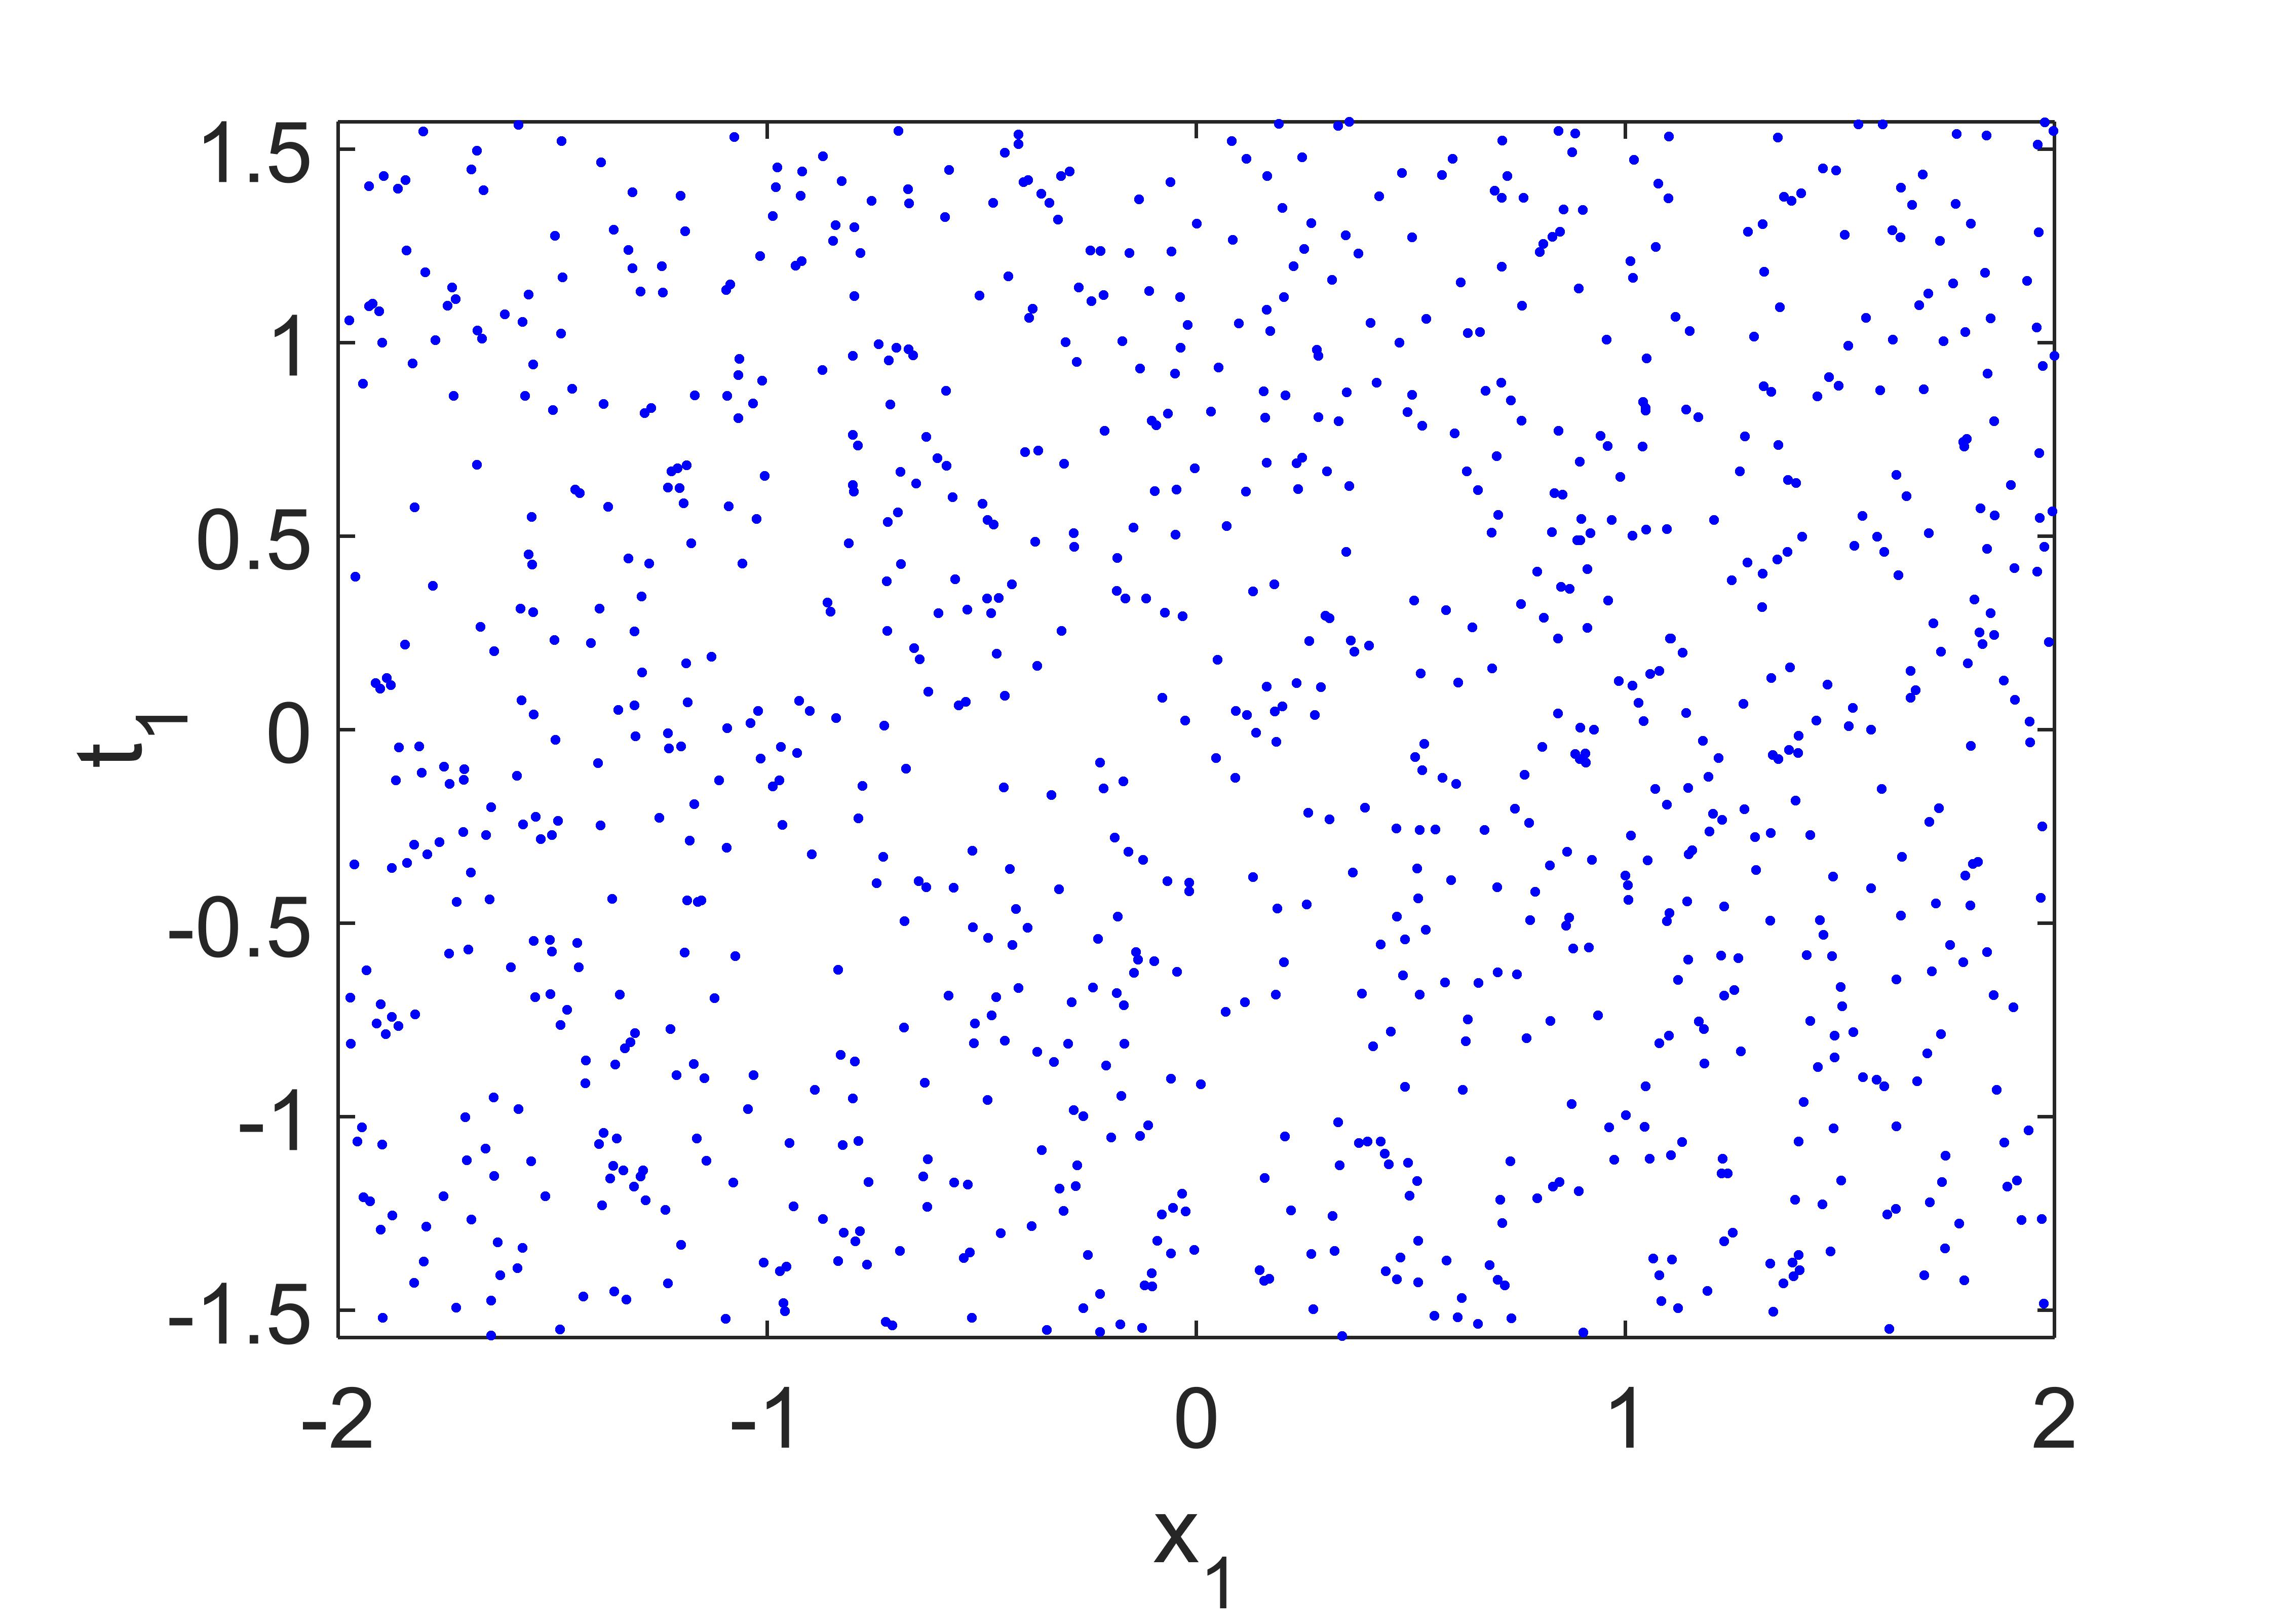
\includegraphics[width=0.8\textwidth]{mc_sample.jpg}
    \caption{Rays at the source of the two-faceted cup with random position coordinate $\variabile{x}$ and random angular coordinates $\optangle$. $10^3$ rays are depicted in this figure.}
    \label{fig:mc_sample1}
\end{center}
  \end{figure}
\\ \indent For the intensity computation we consider a sample of $10^4$ random rays and we divide the target target $\point{T} = [-\variabile{b}, \variabile{b}]$ into $\nbin= 100$ bins.
%Using Eq. (\ref{g_mc}), the normalized intensity $I_{\const{MC}}$ is computed. $I_{\const{MC}}$  is a piecewise constant function, therefore the averaged normalized intensity  $\hat{I}_{\const{MC}}(\optangle_{\variabile{j}-1/2})$ is given considering the values that the intensity $I_{\const{MC}}$ assumes on the middle point $(\optangle_{\variabile{j}-1/2})_{\variabile{j} = 0, \cdots, \nbin}$ of every bin of the partitioning $P_1$. 
The profile of $\hat{I}_{\const{MC}}$ is depicted in Figure \ref{fig:mc_intensity} with the red line. The exact intensity is shown with the green line in the same figure.
\begin{figure}[t]
\begin{center}
    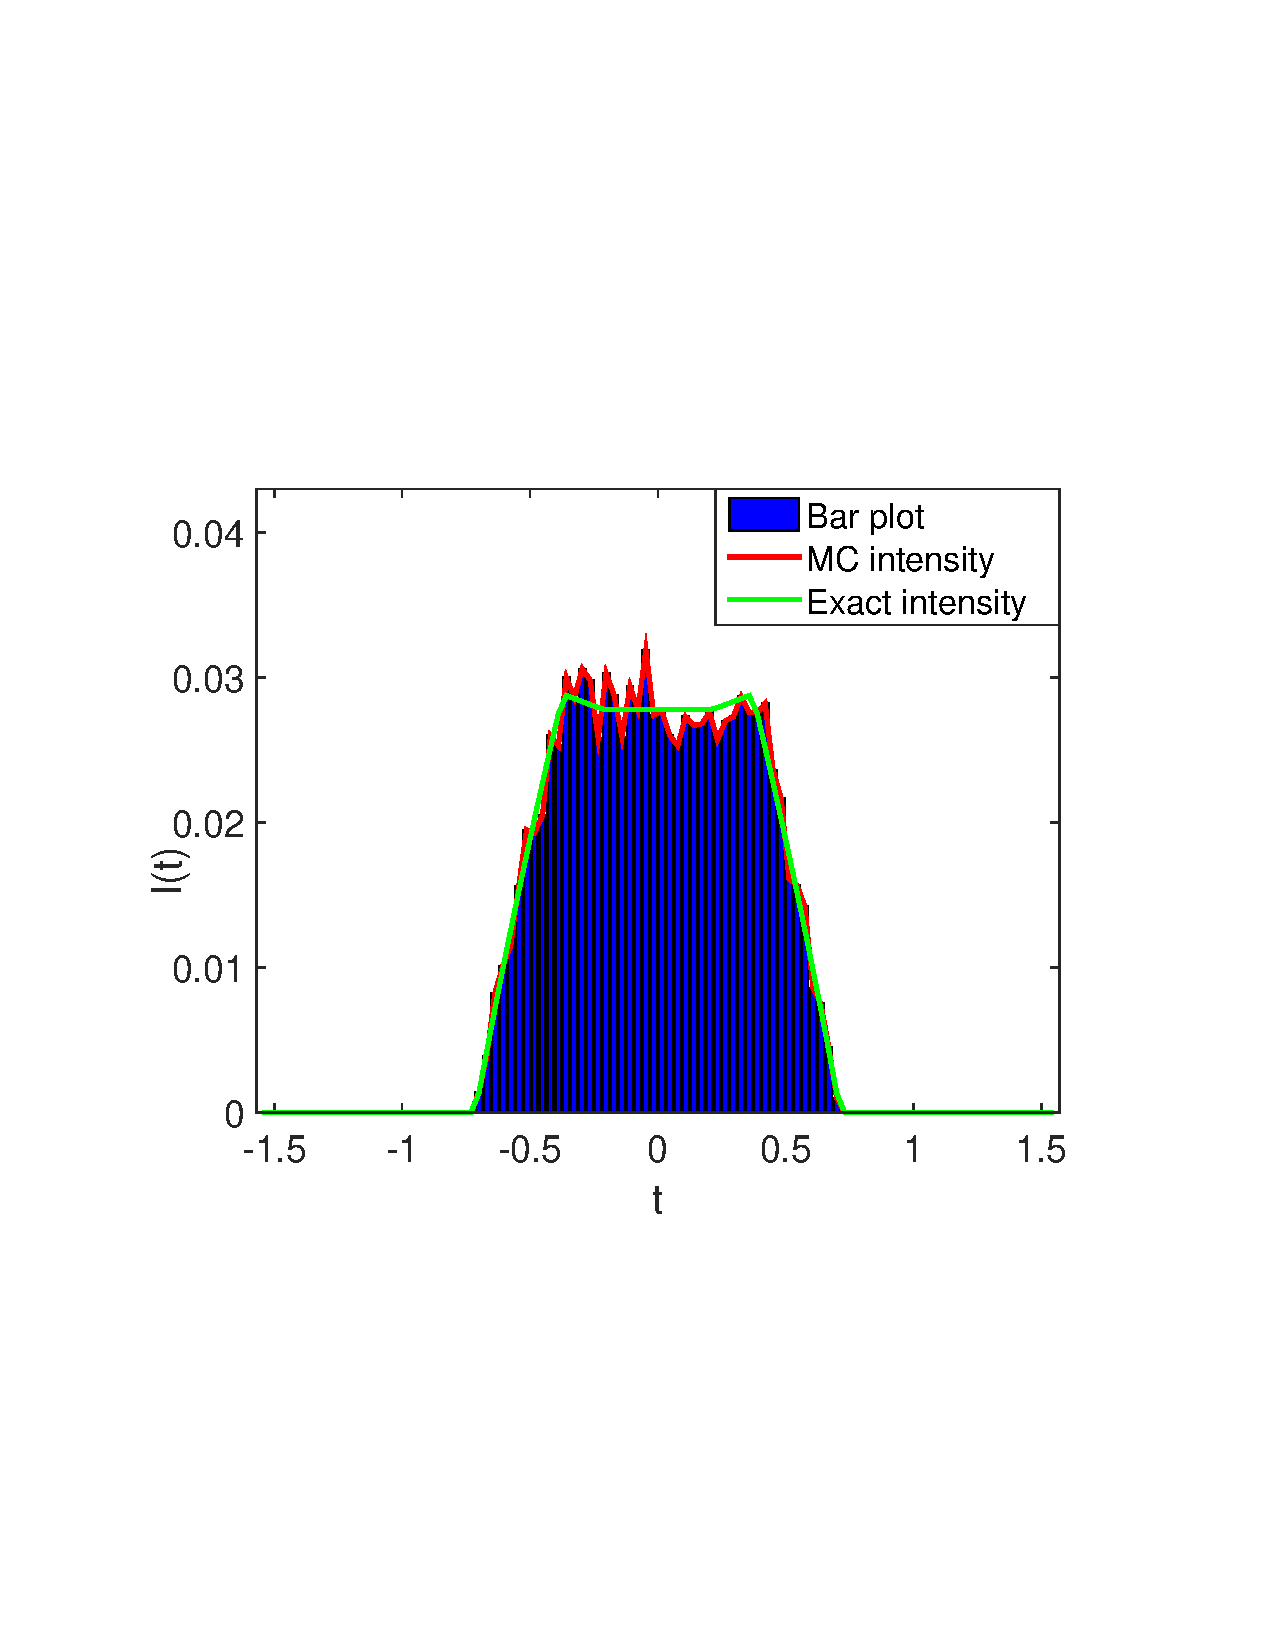
\includegraphics[width=0.8\textwidth]{MC_raytracing.jpg}
    \caption{Comparison between the averaged normalized MC intensity and the normalized exact intensity. The MC intensity is using MC ray tracing with $\nrays = 10^4$ and $\nbin = 100$.}
   \label{fig:mc_intensity}
\end{center}
\end{figure}
MC ray tracing has the advantages of being very easy to implement and it does not require too much regularity of the function that has to be approximated. Furthermore, the error convergence does not depend on the dimension of the domain in which the function is defined.
On the other hand, the MC method is time consuming as the error, for a fixed number of bins, has a speed of convergence of order $O(1/\sqrt{\const{Nr}})$. 
Thus, to decrease the error of a factor $10$ we need to increase the number of rays by a factor $100$.
Since MC ray tracing is a binning procedure, the error depends also on the number of bins in which the target is divided. Finally we remark that the error bound is only a \emph{probabilistic} error as shown in Equation (\ref{eq:mean_error}). This means that, to calculate the value of the error, several simulations have to be repeated and the average of the errors obtained in every simulation has to be calculated. \\ \indent 
The MC noise can be reduced considering a different distribution of the initial rays set.
Instead of considering random variable the sample of rays can be defined such that they are regularly distributed on the domain $D\subseteq\mathbb{R}^2$ of $f$. Methods based on this deterministic approach are called Quasi-Monte Carlo (QMC) methods. The ray tracing procedure that considers such rays distribution is called QMC ray tracing.
\section{Quasi-Monte Carlo ray tracing}\label{sec:QMC}
As in the previous section we first introduce QMC methods and then we briefly explain QMC ray tracing. QMC methods were proposed for the first time in the 1950s in order to speed up MC. Like MC methods, QMC procedures can be used to approximate the integral of a function $f$ using the approximation in (\ref{eq:approx_MC_QMC}).\\ \indent
This section provides basic the notions about uniform distribution theory following the Chapter $2$ of \cite{leobacher2014introduction}. 
It is useful to restrict ourselves to sets of the form $[\vect{a}, \vect{b})= [a_1,b_1)\times[a_2, b_2)\subseteq[0,1)^2$ and introduce the concept of sequences uniformly distributed modulo $1$.
\begin{definition}
An infinite sequence $\{\vect{y}_\variabile{n}\}_{\variabile{n}\in\mathbb{N}_0} \in [0,1)^2$ is said to be \textit{uniformly distributed modulo $1$} (or equidistributed), if for every subset $[\vect{a},\vect{b})\subseteq[0,1)^2$
\begin{equation}
\lim_{N\rightarrow \infty}\frac{\textrm{card}(A([\vect{a},\vect{b}), N))}{N} = \lambda([\vect{a},\vect{b}))
\end{equation}
where $\textrm{card}(A([\vect{a},\vect{b}), N))$ is the cardinality of the following set
\begin{equation}
A([\vect{a},\vect{b}), N) = \{\variabile{n}\in \mathbb{N}_0 | 0\leq\variabile{n}\leq \const{N}-1 \mbox{ and } \vect{y}_{\variabile{n}}\in [\vect{a},\vect{b})\}\,,
\end{equation} that is the number of $\vect{y}_{\variabile{n}}$ such that $\vect{y}_{\variabile{n}}\in [\vect{a},\vect{b})$ and $\lambda([\vect{a},\vect{b})) =(b_1-a_1)\times (b_2-a_2)$.
\end{definition}
Given a sequence $\{\vect{y}_\variabile{i}\}_{\variabile{i} = 1, \cdots, N}\in[0,1)^2$ uniformly distributed modulo $1$ and a 
Riemann integrable function $f:[0,1]^2\rightarrow \mathbb{R}$, the integral of $f$ can be approximated as the average of the values that $f$ assumes on $\{\vect{y}_\variabile{i}\}$ for every $\lineai=\{1, \cdots, N\}$, that is:
\begin{equation}
 \lim_{N\rightarrow \infty}\frac{1}{N}\sum_{\variabile{i}=1}^{N}f(\variabile{y}_{\variabile{i}}) = \int_{[0,1]^2}f(\vect{y})\textrm{d}\vect{y}.
\end{equation}
The idea of QMC methods is to generate the set of points $\vect{y}_{\variabile{i}}$ in $[\vect{a},\vect{b})$ such that they are not randomly distributed but also not exactly uniformly distributed. 
To measure how much the distribution of these points differs from a uniform distribution, the concept of discrepancy was introduced. 
Intuitively, discrepancy measures how much the samples differ from a uniform distribution. 
Therefore, random sequences have a very high discrepancy, while uniformly distributed sequences have zero discrepancy. 
\textit{Low-discrepancy sequences} are sequences with a low discrepancy \cite{owen2003quasi}. A discrepancy of a sequence is \textit{low} if the portion of points of the sequences belonging to an arbitrary set is close to the measure of that set.
The definition of discrepancy in more mathematical terms is provided next. 
\begin{definition}
Given a set $\mathcal{S} = \{\vect{y}_1, \cdots, \vect{y}_\const{N}\}$ of $\const{N}$ points in $[0,1)^2$. The discrepancy $D_\const{N}({\mathcal{S}})$ of $\mathcal{S}$ is defined as
\begin{equation}
D_\const{N}({\mathcal{S}}) = \sup_{\vect{a}, \vect{b}\in[0,1)^2}\Big|\frac{\textrm{card}(A([\vect{a},\vect{b}), \const{N}))}{\const{N}}-\lambda([\vect{a}, \vect{b}))\Big|
\end{equation}
\end{definition}
Often, it is enough to consider the discrepancy in the subset $[\vect{a},\vect{b})\subseteq[0,1)^2$ with $\vect{a}=0$, in which case we talk about star discrepancy.
 \begin{definition}
Let $\mathcal{S} = \{\vect{y}_1, \cdots, \vect{y}_N\}$ be a set of $N$ points in $[0,1)^2$. The  star discrepancy $D^*_N({\mathcal{S}})$ of $\mathcal{S}$ is defined as:
\begin{equation}
D^*_N({\mathcal{S}}) = \sup_{\vect{b}\in[0,1)^2}\Big|\frac{\textrm{card}(A([0,\vect{b}), N))}{N}-\lambda([0, \vect{b}))\Big|.
\end{equation}
%where $\chi_{[0,\point{a})}(\variabile{y}_\variabile{i})$ is the indicator function of $[0,\point{a})\subseteq [0.1)^d$ and $\lambda_d([0, \point{a})) = \prod_{\variabile{j}=1}^d \point{a}_\variabile{j}$ denotes the the $d$-dimensional Lesbegue measure. For intervals of the form $[\point{a}, \point{b})\subseteq [0.1)^d$ we have $\lambda_d([\point{a}, \point{b}))=\prod_{\variabile{j}=1}^{d}(\point{b}_\variabile{j}-\point{a}_\variabile{j})$.
\end{definition}
% Maybe add a picture
%Sequences constructed such that the corresponding star discrepancy is of the order of $\mathcal{O}(\log(N)^2/N)$ for $N\rightarrow\infty$ are called \textit{low-discrepancy sequences}, \cite{owen2003quasi}.
An important result shows that, using a low-discrepancy sequence $\{\vect{y}_{\variabile{i}}\}_{\variabile{i}=1, \cdots, \const{N}}$, the absolute error of a QMC algorithm in two dimensions:
\begin{equation}
\const{err}(f, S_{\const{N}}) =\Bigg|\int_{[0,1)^2}f(\vect{y}) \textrm{d}\vect{y}-\frac{1}{\const{N}}\sum_{\variabile{i}=1}^{\const{N}}f(\vect{y}_\variabile{i})\Bigg|
\end{equation}
 can be bounded by the product of a term that depends on $f$ and another term that depends on the discrepancy of the set $\{\vect{y}_{\variabile{i}}\}_{\variabile{i}=1, \cdots, N}.$ This is the result provided by the Koksma-Hlawka inequality which gives the following estimation of the error:
\begin{equation}\label{eq:QMC_error}
|\const{err}(f, S_{N})|= \Bigg|\int_{[0,1)^2}f(\vect{y}) \textrm{d}\vect{y}-\frac{1}{N}\sum_{\variabile{i}=1}^{N}f(\vect{y}_\variabile{i})\Bigg|\leq V(f)D^*_N({\mathcal{S}}),
\end{equation}
% Explain better the variation function owen2005multidimensional
where $V(f)$ is the so-called variation function of $f$ in the sense of Hardy-Krause (see \cite{brandolini2013koksma} for details). 
The previous equation shows that for a function $f$ with finite variation $V(f)$ QMC methods performs much better than MC. However, Equation (\ref{eq:QMC_error}) is not good for predicting when this will happen because $V(f)$ is hard to estimate and in some cases is infinite \cite{wang2008low}. 
%Schlier [32] reports that even for QMC the variance of f is more strongly related to the error than is the variation.
For the functions we analyze in this thesis the corresponding variation function is always bounded. 
The convergence of QMC methods strongly depends on the low-discrepancy sequence that is used.\\ \indent
There are many ways to generate low-discrepancy sequences \cite{dalal2008low}. The most common QMC approach uses the so-called Sobol sequence. The algorithm for generating Sobol sequences is widely explained in the literature, (see for instance \cite{bratley1988algorithm}). In appendix \ref{app:Sobol} we give an overview of how these kind of sequences can be constructed. When using Sobol sequences QMC error can be estimated by:
\begin{equation}
\const{err}(f, S_{N})<C \frac{\log(N)^2}{N}, 
\end{equation}
for some $C>0$.
For higher dimensions $d>2$, the general relation holds
\begin{equation}
\const{err}(f, S_{N})<C \frac{\log(N)^d}{N}.
\end{equation}
%For small dimensions, QMC performs much better than MC methods, while for large dimension the factor $\log(\const{N})$ could be very big. 
% In the following we show a particular construction of a low-discrepancy sequence for $d=1$ that was introduced the first time by Van der Corput in 1935.  
%This kind of sequences, called \textit{van der Corput} sequences, are particular interesting not only because they give an intuition of how to construct low discrepancy sequences but also because many other kind of sequences in higher dimensions are based on this one-dimensional case. Before introducing these sequences we need to give the concept of radical inverse function. Let $\const{b}\geq 2$ be an integer base. Any natural number $\variabile{n}\in \mathbb{N}_0$ can be decomposed in base $\const{b}$ as follows:
%\begin{equation}
%\variabile{n} = \sum_{\variabile{i}=0}^\infty \variabile{d}_{\variabile{i}}\const{b}^{\variabile{i}}
%\end{equation}
%where $\variabile{d}_{\variabile{i}} \in \{0, 1, \cdots, \const{b}-1\}$ are the digit numbers.
%The radical inverse function $\phi_{\const{b}}:\mathbb{N}_0\mapsto [0,1)$ in base $\const{b}$ is defined as:
%\begin{equation}
%\phi_{\const{b}}(\variabile{n}) = \sum_{\variabile{i}=1}^{\infty}\frac{\variabile{d}_{\variabile{i}-1}}{\const{b}^{\variabile{i}}}.
%\end{equation}
%As an example we provide in the following the radical inverse function $\phi_{\const{b}}(5)$ in base $\const{b} = 2$. 
%The digit expansion in base $\const{b}$ of $\variabile{n}=5$ is:
%\begin{equation}
%5 = 1\cdot 2^0+1\cdot 2^2.
%\end{equation}
%Therefore, $\variabile{d}_0 = 1, \variabile{d}_1 = 0$ and $\variabile{d}_2 = 1$. 
%The radical inverse function $\phi_2(5)$ is:
%\begin{equation}
%\phi_2 (5) = \frac{1}{2}+\frac{1}{8} = \frac{5}{8}.
%\end{equation}
%\begin{definition}
%The Van der Corput sequence in base $\const{b}$ is defined as $\{ \phi_{\const{b}}(\variabile{n})\}_{n\in\mathbb{N}_0}$.
%\end{definition}
%For example, suppose we have the finite sequence of numbers $\variabile{n}\in \{0, 1,\cdots, 8\}$  the corresponding Van der Corput sequence 
%$\{ \phi_{\const{b}}(\variabile{n})_{\variabile{n}\in \{0, 1,\cdots, 8\}}$ in base $\variabile{b}=2$ is:
%\begin{equation}
%\big\{\phi_2(\variabile{n})\big\}_{\variabile{n}\in \{0, 1,\cdots, 8\}} = \Bigg\{0, \frac{1}{2}, \frac{1}{4}, \frac{3}{4}, \frac{1}{8},\frac{5}{8}, \frac{3}{8}, \frac{7}{8}, \frac{1}{16}\Bigg\} \,.
%\end{equation}
%It can be proved that the Van der Corput sequence in base $\variabile{b}$ is uniformly distributed modulo one, \cite{leobacher2014introduction}. 
%The van der Corput sequence has been extended to higher dimensions. 
%The most common QMC approach uses Sobol sequence which is one an extended Van der Corput sequence in base $\variabile{b}=2$ to $\variabile{d}\geq2$. 
\\ \indent Ray tracing based on QMC methods considers as position and angular coordinates of the rays at the source, the coordinates of the corresponding points of a low-discrepancy sequence. 
Therefore, to implement QMC ray tracing in two-dimensions we need to construct a low-discrepancy sequence in two-dimensions.  
Given, for instance, a Sobol sequence $\{\vect{y}_{\variabile{i}}\}_{\variabile{i}=1, \cdots, N}$ with $\vect{y}_\variabile{i}\in[0,1)^2$ for every $\variabile{i}=1, \cdots, N$, the two dimensional QMC ray tracing the coordinates $(\variabile{x}_1^{\variabile{i}}, \optangle_1^{\variabile{i}})$ of the $\variabile{i}$-th ray at the source equal to those of the $\variabile{i}$-th points of the sequence, i.e., $(\variabile{x}_1^{\variabile{i}}, \optangle_1^{\variabile{i}})=\vect{y}_{\variabile{i}}$. A set of $\nrays = N$ rays with these initial coordinates is traced within the system and the target coordinates of all the rays traced are computed. \\ \indent 
Similarly to MC ray tracing, the averaged and normalized QMC intensity $\hat{I}_{\const{MC}}$ is given by the approximation in (\ref{eq:approx_MC_QMC}), where now the variable $\vect{y}$ is a variable of the Sobol sequence instead of a random variable. Therefore, the target is divided into $\nbin$ bins and the averaged number of rays that follow into each bin is considered. The intensity is still a piecewise constant function, and its value over every bin $[\optangle_{\variabile{j}-1}, \optangle_{\variabile{j}})_{\variabile{j}=1, \cdots, \nbin}$ is given by the intensity $I(\optangle_{\variabile{j}-1/2})$ calculated along the direction $\optangle_{\variabile{j}-1/2}$ (middle point of the bin). The only difference between MC and QMC ray tracing consists on the choice of the initial ray set. Thus, we expect that QMC and MC ray tracing have the same dependence of the error as a function of the number of bins $\nbin$. More precisely, since the discretization error (first term on the right hand side of inequality (\ref{eq:error_int})) does not depend on MC noise, we expect that it does not change for QMC error. Regarding the second terms on the right hand side of inequality (\ref{eq:error_int})), we showed in the previous section that it depends on the standard deviation of the approximated intensity $\hat{I}_{\const{MC}}$ and on the number of bins. Hence, indicating with $I(\optangle_{\variabile{j}-1/2})$ the exact value of the intensity at direction $\optangle_{\variabile{j}-1/2}$, we can predict that the QMC error over every bin is estimated by:
\begin{equation} \begin{aligned}
\Big|I(\optangle_{\variabile{j}-1/2})&-\frac{\Phi}
{\Delta\optangle}I_{\const{QMC}}(\optangle_{\variabile{j}-1/2})\Big| \leq
\frac{\const{C}_1}{\nbin^2} + \const{C}_2\nbin\frac{\log(\nrays-\nbin)^2}{\nrays},
\end{aligned}
\end{equation}
for some $C_1>0$ and $C_2>0$.
\\ \indent
In Figure \ref{fig:qmc_sample1} we show the distribution of the position and direction coordinates of the rays at the source of the two-faceted cup in Figure \ref{fig:cup}. 
A set of $10^3$ rays generated from a $2D$ Sobol sequence is considered, the coordinates $(\variabile{x}_1, \optangle_1)$ of every ray at the source are depicted with blue dots.
We note that the rays have a regular distribution on the $(\variabile{x}, \optangle)$-plane.
We need to remark that, for the system in Figure \ref{fig:cup}, $\variabile{x}_1 \in[-2,2]$ and the angular coordinates $\optangle_1 \in[-\pi/2, \pi/2]$. 
Since Sobol sequences are defined inside intervals of the  $[\vect{a}, \vect{b})\subseteq[0,1)^2$, we scaled the points of the sequence $\vect{y}_{\variabile{i}}$ in order to take all the possible positions and directions that the rays can assume at the source, therefore, for this system, $\variabile{x}_1^{\variabile{i}} = -2+4\,y_{\variabile{i}}(1)$ and $\optangle_1^{\variabile{i}} = -\pi/2+\pi\,y_{\variabile{i}}(2)$ where 
$\vect{y}_{\variabile{i}} = \big(y_{\variabile{i}}(1), y_{\variabile{i}}(2)\big)$ is a point of the Sobol sequence. 
\begin{figure}[t]
\begin{center}
    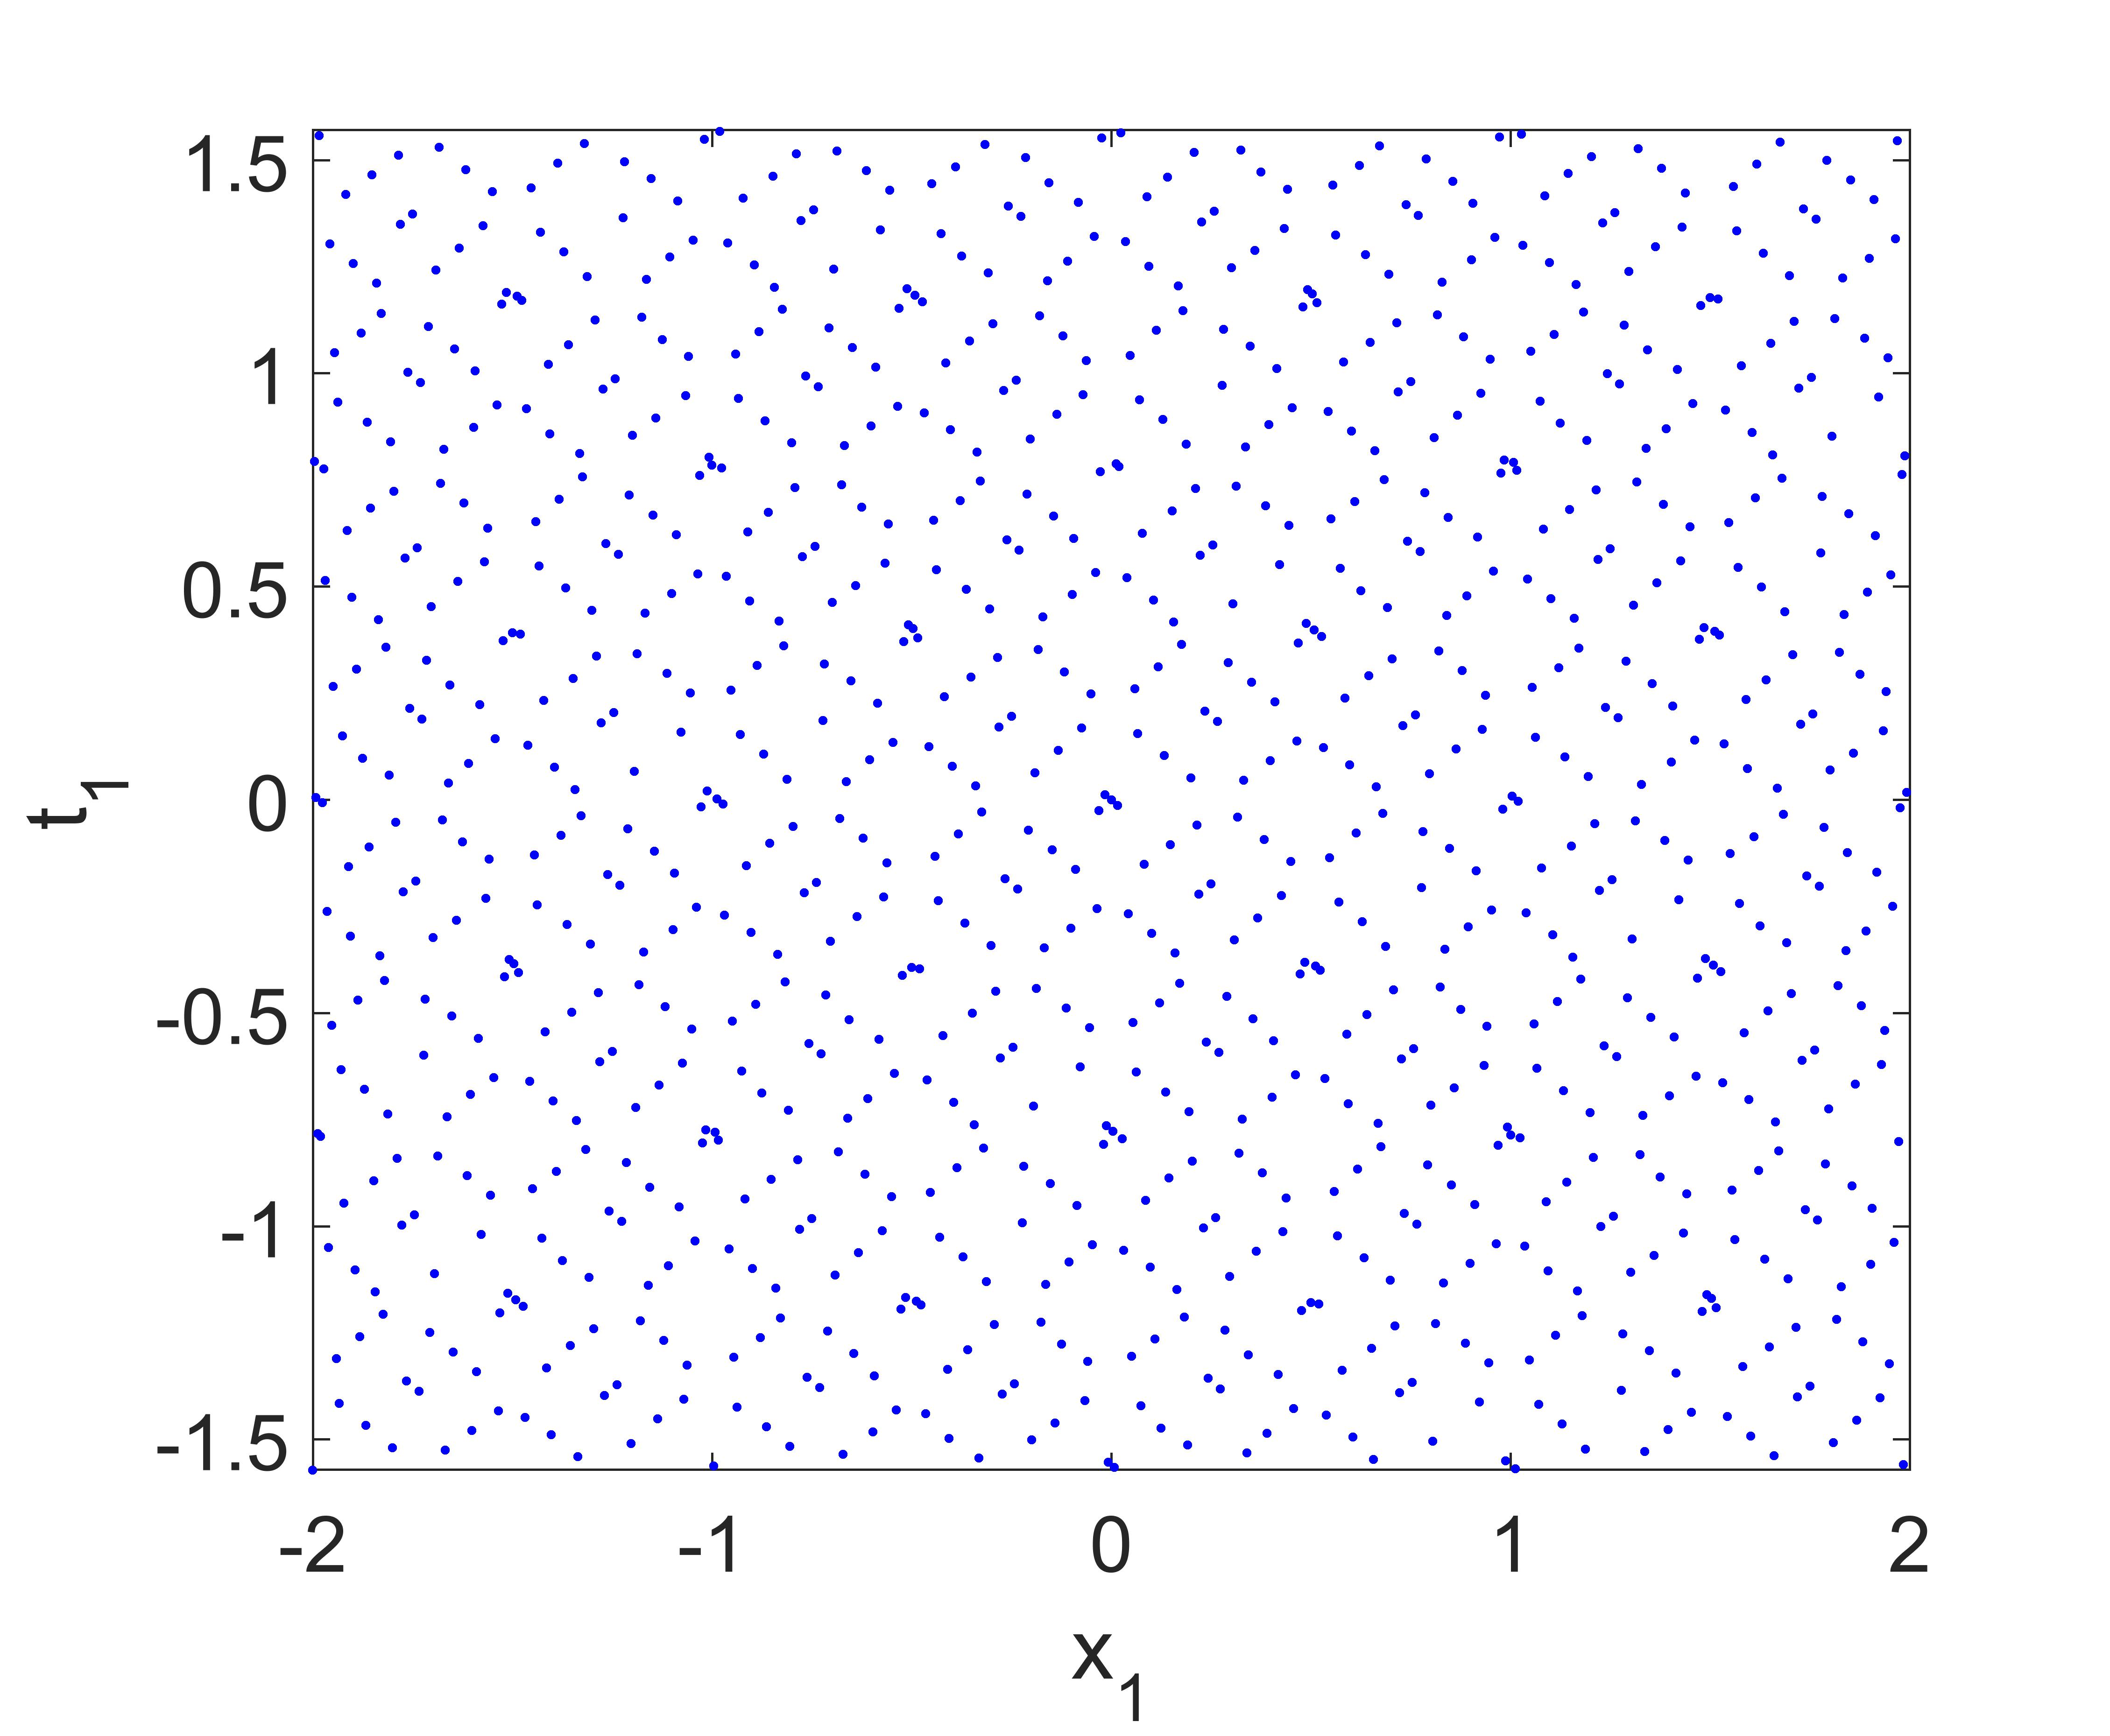
\includegraphics[width=0.8\textwidth]{qmc_sample.jpg}
    \caption{$10^3$ rays at the source of the two-faceted cup with position coordinate $\variabile{x}_1$ and angular $\optangle_1$ coordinate with a regular distributions.
They are distributed as the points of a Sobol sequence in two-dimensions.}
    \label{fig:qmc_sample1}
\end{center}
  \end{figure}
\\ \indent Dividing the target into $\nbin=100$ bins, we computed the target intensity. 
In Figure \ref{fig:qmc_intensity} we show the profile of the output intensity at the target of the two-faceted cup computed using QMC ray tracing with $10^4$ rays. 
The QMC intensity is depicted with the red line. It is compared to the exact intensity shown in the same figure with the green dotted line.
A comparison between Figure \ref{fig:mc_intensity} and \ref{fig:qmc_intensity} shows that for the two-faceted cup and for a set of $\nrays=10^4$ rays, QMC ray tracing performs better than MC ray tracing. In order compare MC and QMC ray tracing, we calculate the target intensity using both methods gradually increasing the number of rays traced inside the two-faceted cup. The errors between the approximated averaged normalized intensity $\hat{I}_{\textrm{A}} (\textrm{A} = \textrm{MC}, \textrm{QMC})$ and the exact normalized intensity $\hat{I}_\textrm{exact}$ are calculated.
% Explain the speed of convergence
The speed of convergence for MC is shown in Figure \ref{fig:Error_cup} with the red, while the behavior of QMC ray tracing is depicted in the same picture with the blue line.
The results shown for a simple optical system are indeed consistent with what we expected from the theoretical analysis.
\\\indent Although QMC ray tracing is an improvement of MC ray tracing for small dimensions, it has two main disadvantages. 
First, its convergence is strongly related with the dimension in which it is implemented.
Second, likewise MC ray tracing, QMC ray tracing is a binning procedure, therefore the error still depends on the number of bins in which the target is divided and only the averaged value of the intensity over every bin is provided.
\begin{figure}[t]
\begin{center}
    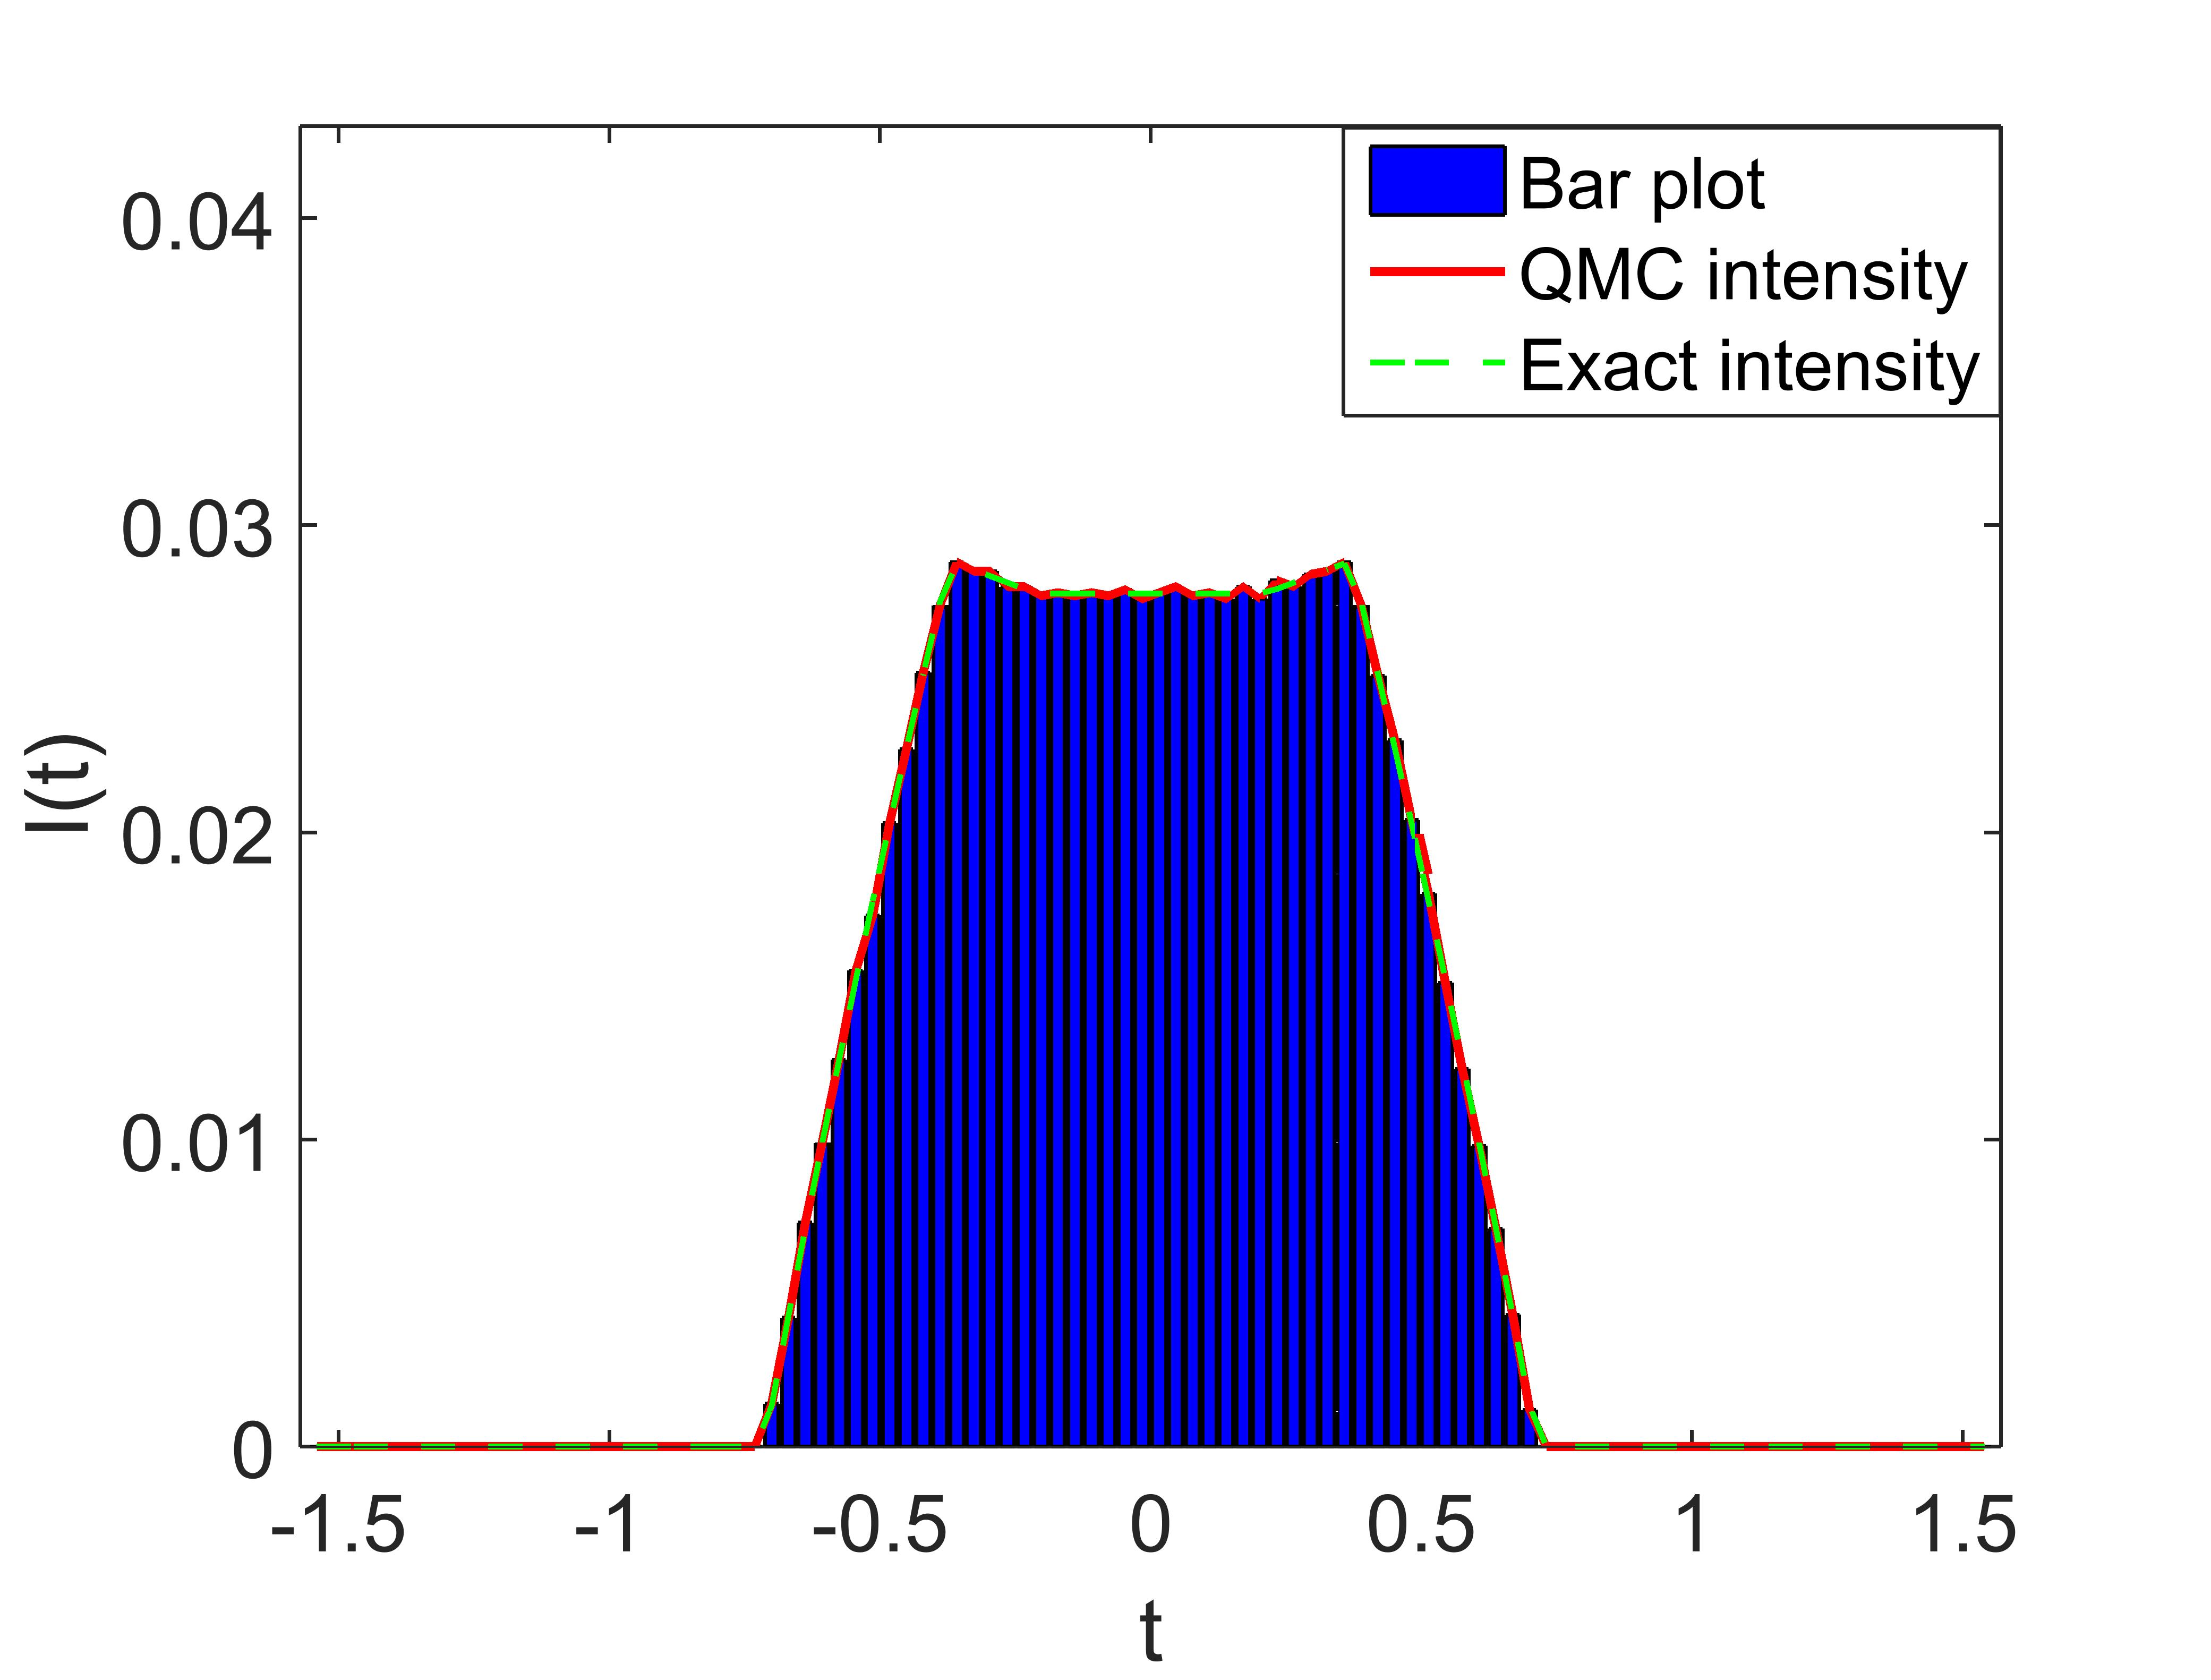
\includegraphics[width=0.8\textwidth]{qmc_raytracing.jpg}
    \caption{QMC intensity for the two-faceted cup obtained tracing $\nrays=10^4$ rays and dividing the target into $\nbin=100$ bins.}
    \label{fig:qmc_intensity}
\end{center}
  \end{figure}
\begin{figure}[h]
\begin{center}
    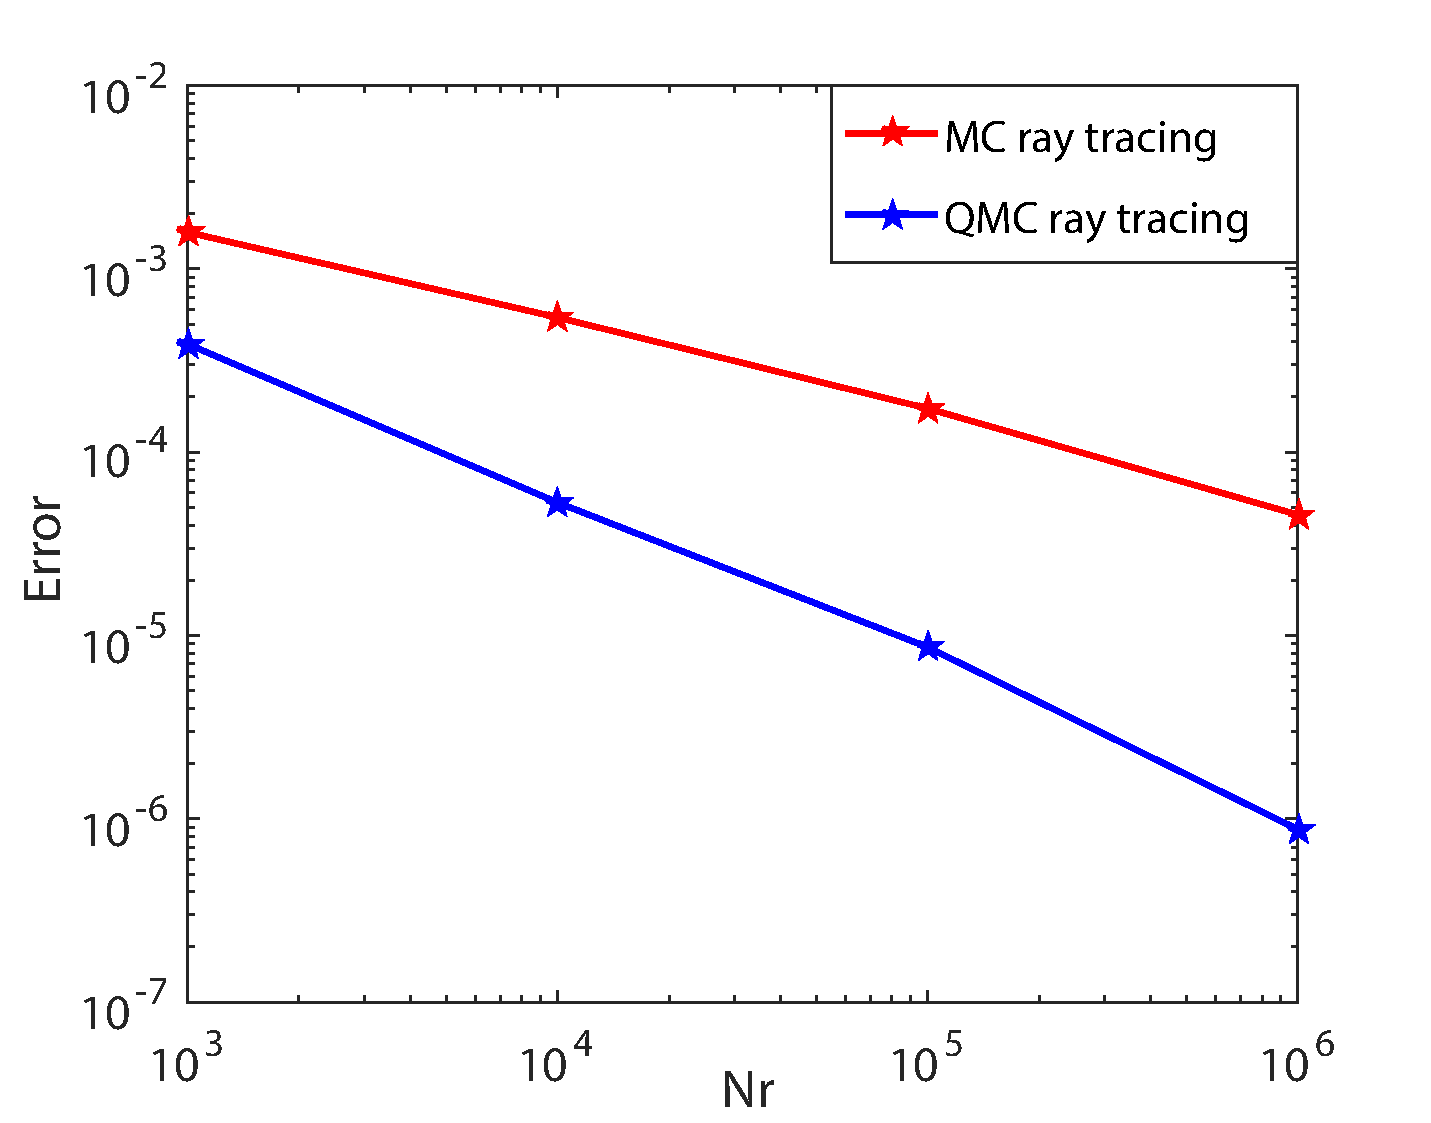
\includegraphics[width=0.8\textwidth]{Error_cup}
    \caption{Error as function of the number of rays traced in a logarithmic scale for fixed number of bins $\nbin=100$.
 MC ray tracing convergence is of the order $\mathcal{O}(1/\sqrt{\nrays})$ and it is shown with the red line. 
QMC ray tracing convergence is of the order $\mathcal{O}(1/\nrays)$ and it is depicted with the blue line.}
    \label{fig:Error_cup}
\end{center}
  \end{figure}
 \\\ \indent
From the results provided in this chapter we can conclude that the choice of the initial ray set can make a big impact on the performance of the ray tracing procedure. 
Based on the idea of taking a smart choice of the initial ray set, we develop a new ray tracing method which is based on phase space. 
The phase space (PS) concept will be introduced in the next chapter. The new ray tracing method employs the PS of the source and the target of the optical systems.
We will show that phase space ray tracing allows to trace a relatively small number of rays inside the system to obtain the desired accuracy of the target intensity. 





















